\documentclass[12pt]{article}

\pdfobjcompresslevel=3    % compress PDF objects
\pdfcompresslevel=9       % compress streams more (0..9)
\pdfminorversion=4

\usepackage[utf8]{inputenc}
\usepackage[T1]{fontenc}

% Layout & graphics
\usepackage[a4paper, total={7.5in, 9in}]{geometry}
\usepackage{graphicx}              % images
\usepackage[dvipsnames,table]{xcolor} % single xcolor invocation

% Math & symbols
\usepackage{amsmath}
\usepackage{amssymb}
\usepackage{gensymb}
\usepackage{array}

% Typography & layout helpers
\usepackage{microtype}
\usepackage{float}                 % [H] placement
\usepackage{caption}
\usepackage{subcaption}
\usepackage{multirow}
\usepackage{titlesec}
\usepackage{lmodern}

\definecolor{xppblue}{RGB}{37, 150, 190}

\begin{document}

\begin{table}[H]
\centering
\begin{tabular}{|m{4cm}|m{8cm}|m{2cm}|}
\hline
\multicolumn{2}{|c|}{\cellcolor{xppblue}\textcolor[rgb]{1,1,1}{Politechnika Poznańska}}  & \multicolumn{1}{c|}{\multirow{3}{*}{\resizebox{14mm}{!}{
\includegraphics{images/logo.png}}}}\\ 
\multicolumn{2}{|c|}{\cellcolor{xppblue}\textcolor[rgb]{1,1,1}{Wydział Automatyki, Robotyki i Elektrotechniki}} & \\ 
\multicolumn{2}{|c|}{\cellcolor{xppblue}\textcolor[rgb]{1,1,1}{Instytut Robotyki i Inteligencji Maszynowej}} & \\ 
\hline 
\multicolumn{1}{|c|}{Dz>AiR>Sem6} & \multicolumn{1}{c|}{Automatyka układów napedowych} & \multicolumn{1}{c|}{2025/26 (s.letni)} \\
\hline
 Jan Andrzejewski \par Mateusz Banaszak & \large{\textbf{Zaawansowane metody komutacji w napędzie BLDC}} & Data wyk.:\par 01.04.2026 \\
\hline
Grupa L8  &  &  \\
\hline
\end{tabular}
\end{table} 


\section{Sterowanie dwiema metodami komutacji}

\subsection{Sterowanie trapezowe bezczujnikowe (kąt 120 stopni)}

Sterowanie trapezowe o kącie przewodzenia $120^{\circ}$ elektrycznych polega na zasilaniu w danej chwili 
tylko dwóch z trzech faz silnika. Trzecia faza pozostaje w stanie bezprądowym (przez $60^{\circ}$ w każdej półfali), 
co w metodach bezczujnikowych ułatwia detekcję położenia wirnika na podstawie indukowanej siły elektromotorycznej (Back-EMF). 
Główne sygnały sterujące komutacją zmieniają się skokowo co $60^{\circ}$ elektrycznych.

Wdrożona w modelu metoda jest w rzeczywistości układem hybrydowym. Ze względu na to, że przy zerowej i bardzo niskiej prędkości obrotowej indukowana siła elektromotoryczna jest zbyt mała do poprawnej detekcji, układ startuje wykorzystując sygnały z czujników Halla. Po przekroczeniu zdefiniowanej prędkości progowej (\texttt{omega\_min}), system automatycznie przełącza się na sterowanie bezczujnikowe bazujące na przecięciach zera przez BEMF. W Tabeli 1 przedstawiono zdefiniowane sygnały sterujące realizujące tę logikę.

\begin{table}[H]
\centering
\renewcommand{\arraystretch}{1.6}
\small
\begin{tabular}{|c|m{13.5cm}|}
\hline
\rowcolor{gray!20}
\textbf{Klucz} & \textbf{Zdefiniowany sygnał sterujący (Równanie LTspice)} \\
\hline
$K_1$ (Górny U) & \texttt{V=if( V(omega)<omega\_min, if(V(H1)>0 \& V(H3)<1, 1, 0), \newline if(V(SEMA)>0 \& V(SEMC)<0, 1, 0) )} \\
\hline
$K_4$ (Dolny U) & \texttt{V=if( V(omega)<omega\_min, if(V(H1)<1 \& V(H3)>0, 1, 0), \newline if(V(SEMA)<0 \& V(SEMC)>0, 1, 0) )} \\
\hline
$K_3$ (Górny V) & \texttt{V=if( V(omega)<omega\_min, if(V(H2)>0 \& V(H1)<1, 1, 0), \newline if(V(SEMB)>0 \& V(SEMA)<0, 1, 0) )} \\
\hline
$K_6$ (Dolny V) & \texttt{V=if( V(omega)<omega\_min, if(V(H2)<1 \& V(H1)>0, 1, 0), \newline if(V(SEMB)<0 \& V(SEMA)>0, 1, 0) )} \\
\hline
$K_5$ (Górny W) & \texttt{V=if( V(omega)<omega\_min, if(V(H3)>0 \& V(H2)<1, 1, 0), \newline if(V(SEMC)>0 \& V(SEMB)<0, 1, 0) )} \\
\hline
$K_2$ (Dolny W) & \texttt{V=if( V(omega)<omega\_min, if(V(H3)<1 \& V(H2)>0, 1, 0), \newline if(V(SEMC)<0 \& V(SEMB)>0, 1, 0) )} \\
\hline
\end{tabular}
\caption{Definicja hybrydowych sygnałów sterujących dla bezczujnikowej metody $120^{\circ}$.}
\label{tab:klucze_120}
\end{table}

Poniżej zaprezentowano wyniki symulacji dla tej metody. 


\begin{figure}[H]
    \centering
    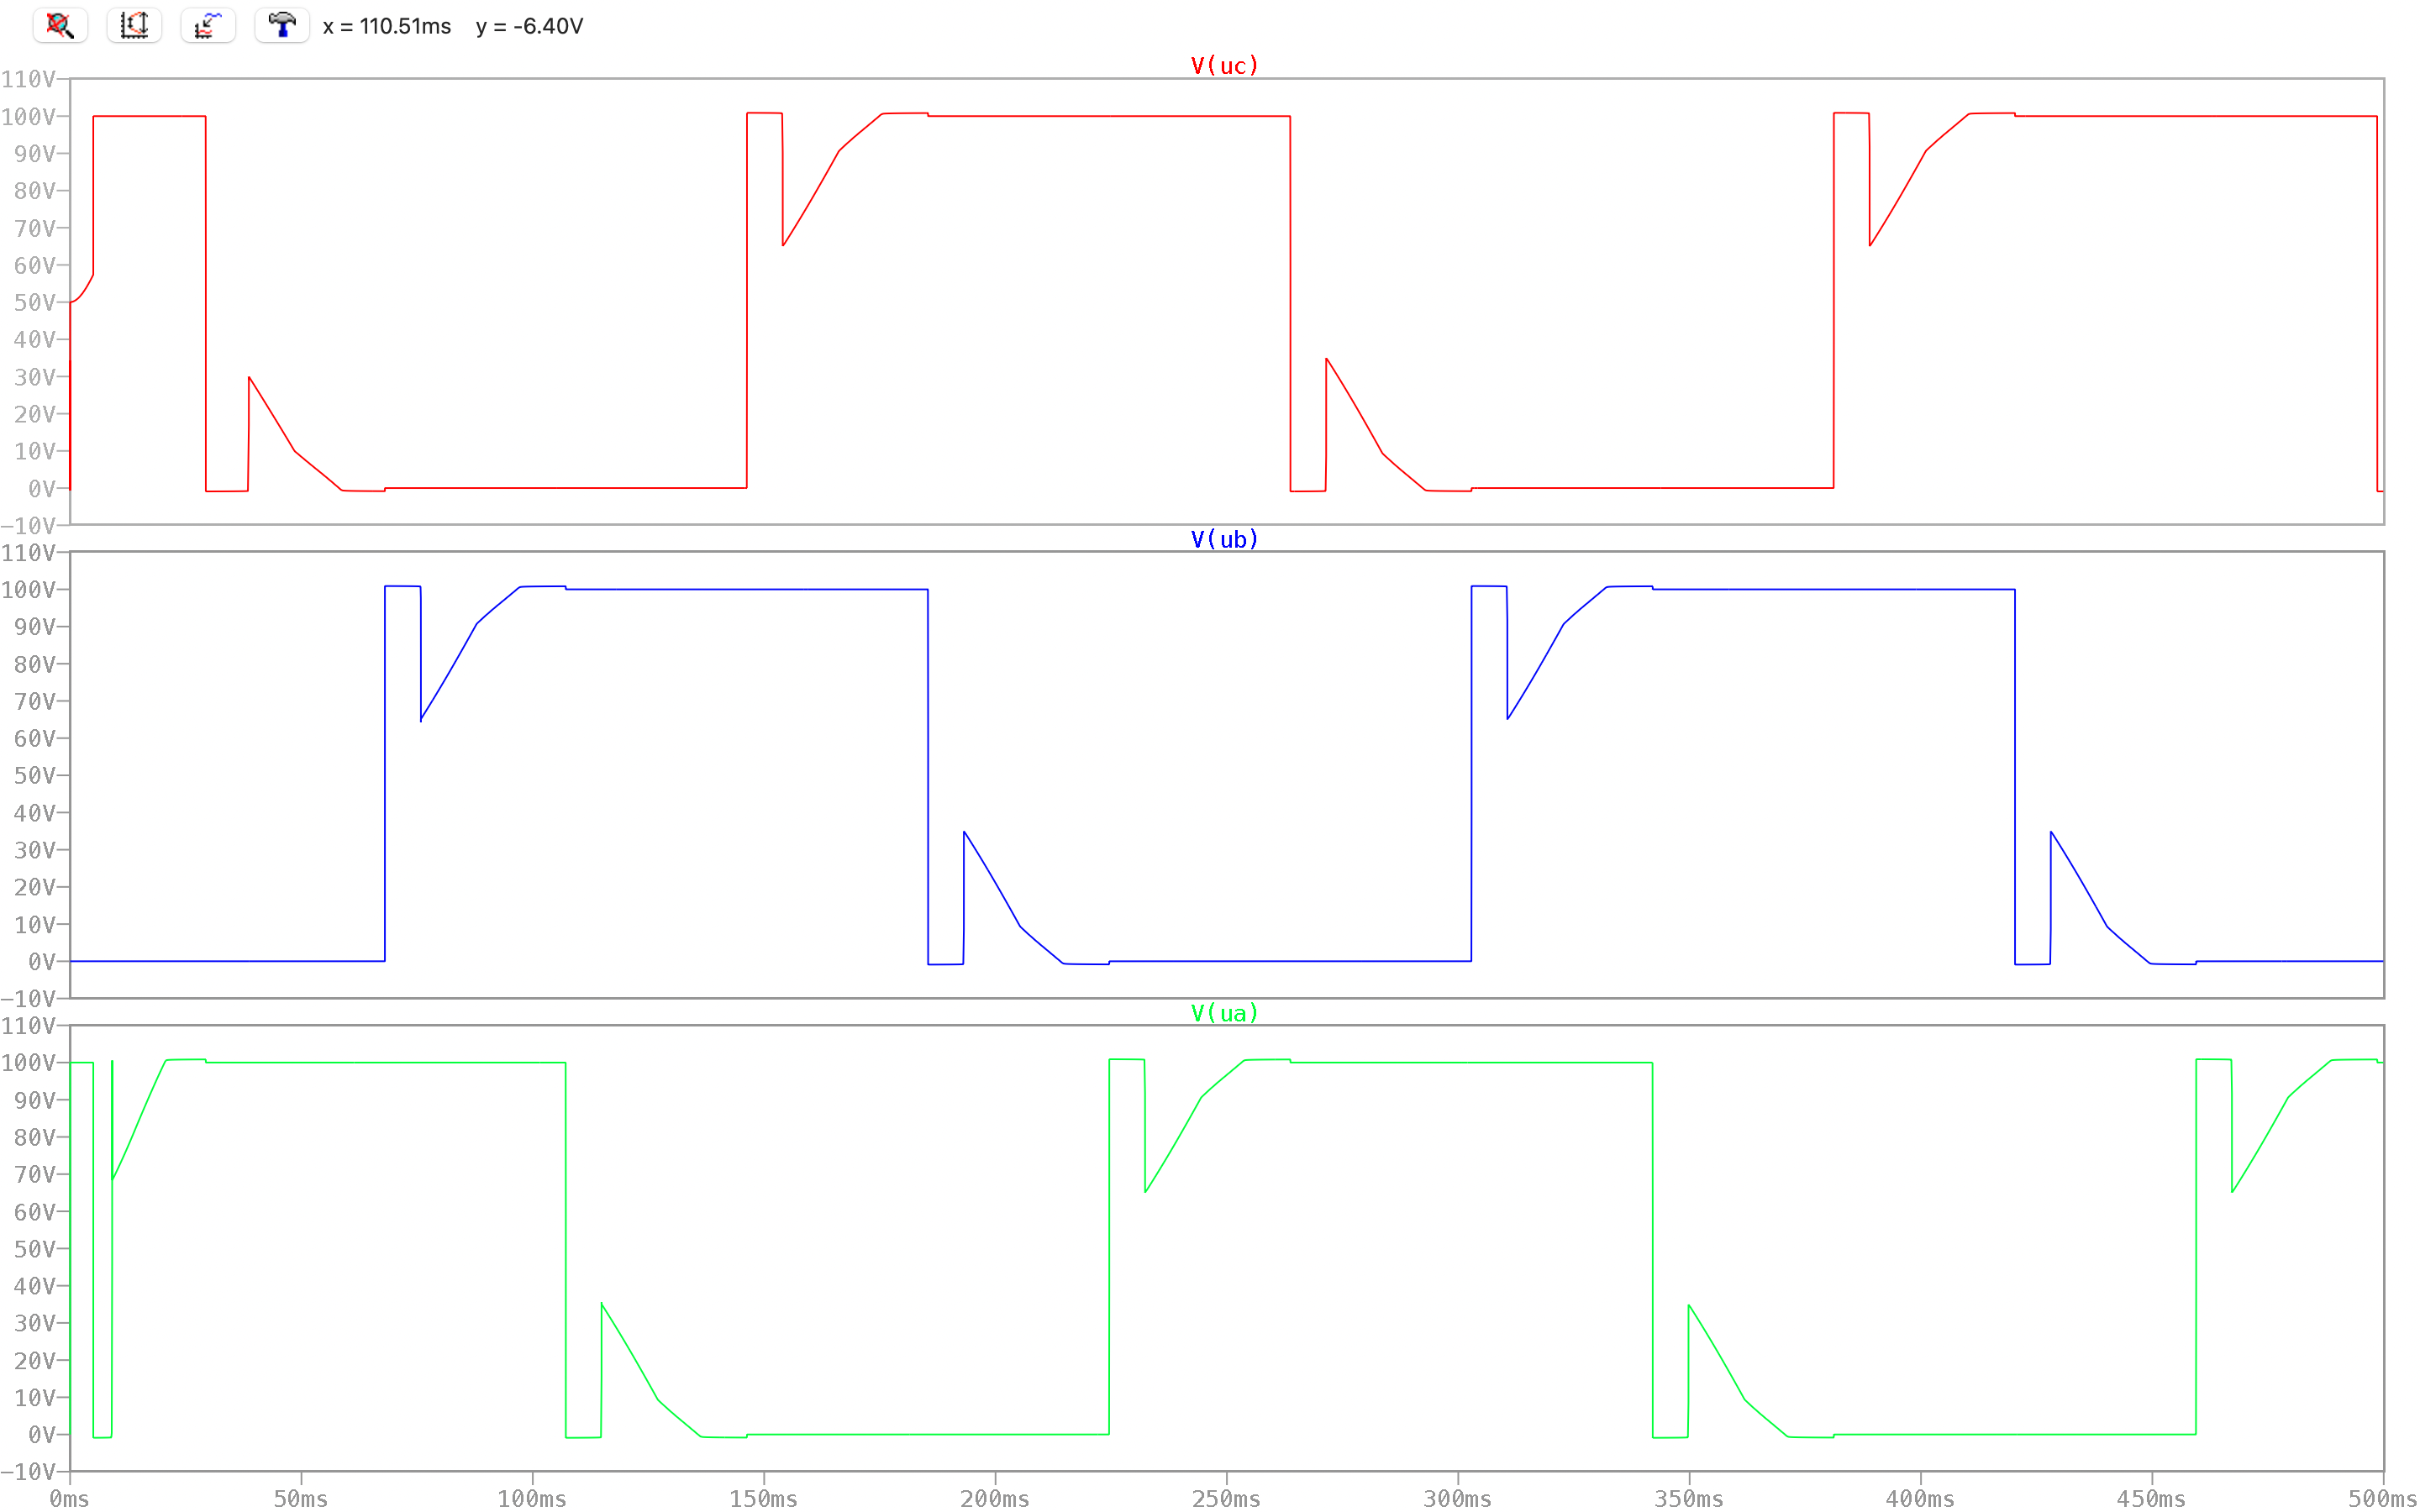
\includegraphics[width=0.8\textwidth]{images/napiecie_fazowe_bezczujnikowo.png}
    \caption{Wykresy napięć fazowych dla sterowania bezczujnikowego $120^{\circ}$}
    \label{fig:120_napiecia_faza}
\end{figure}
Wykresy napięć fazowych charakteryzują się wyraźnymi spłaszczeniami w momentach, gdy dana faza nie jest zasilana z falownika. W tych krótkich przedziałach czasu (trwających po $60^{\circ}$) widoczna jest mierzona indukowana na uzwojeniach siła elektromotoryczna.

\begin{figure}[H]
    \centering
    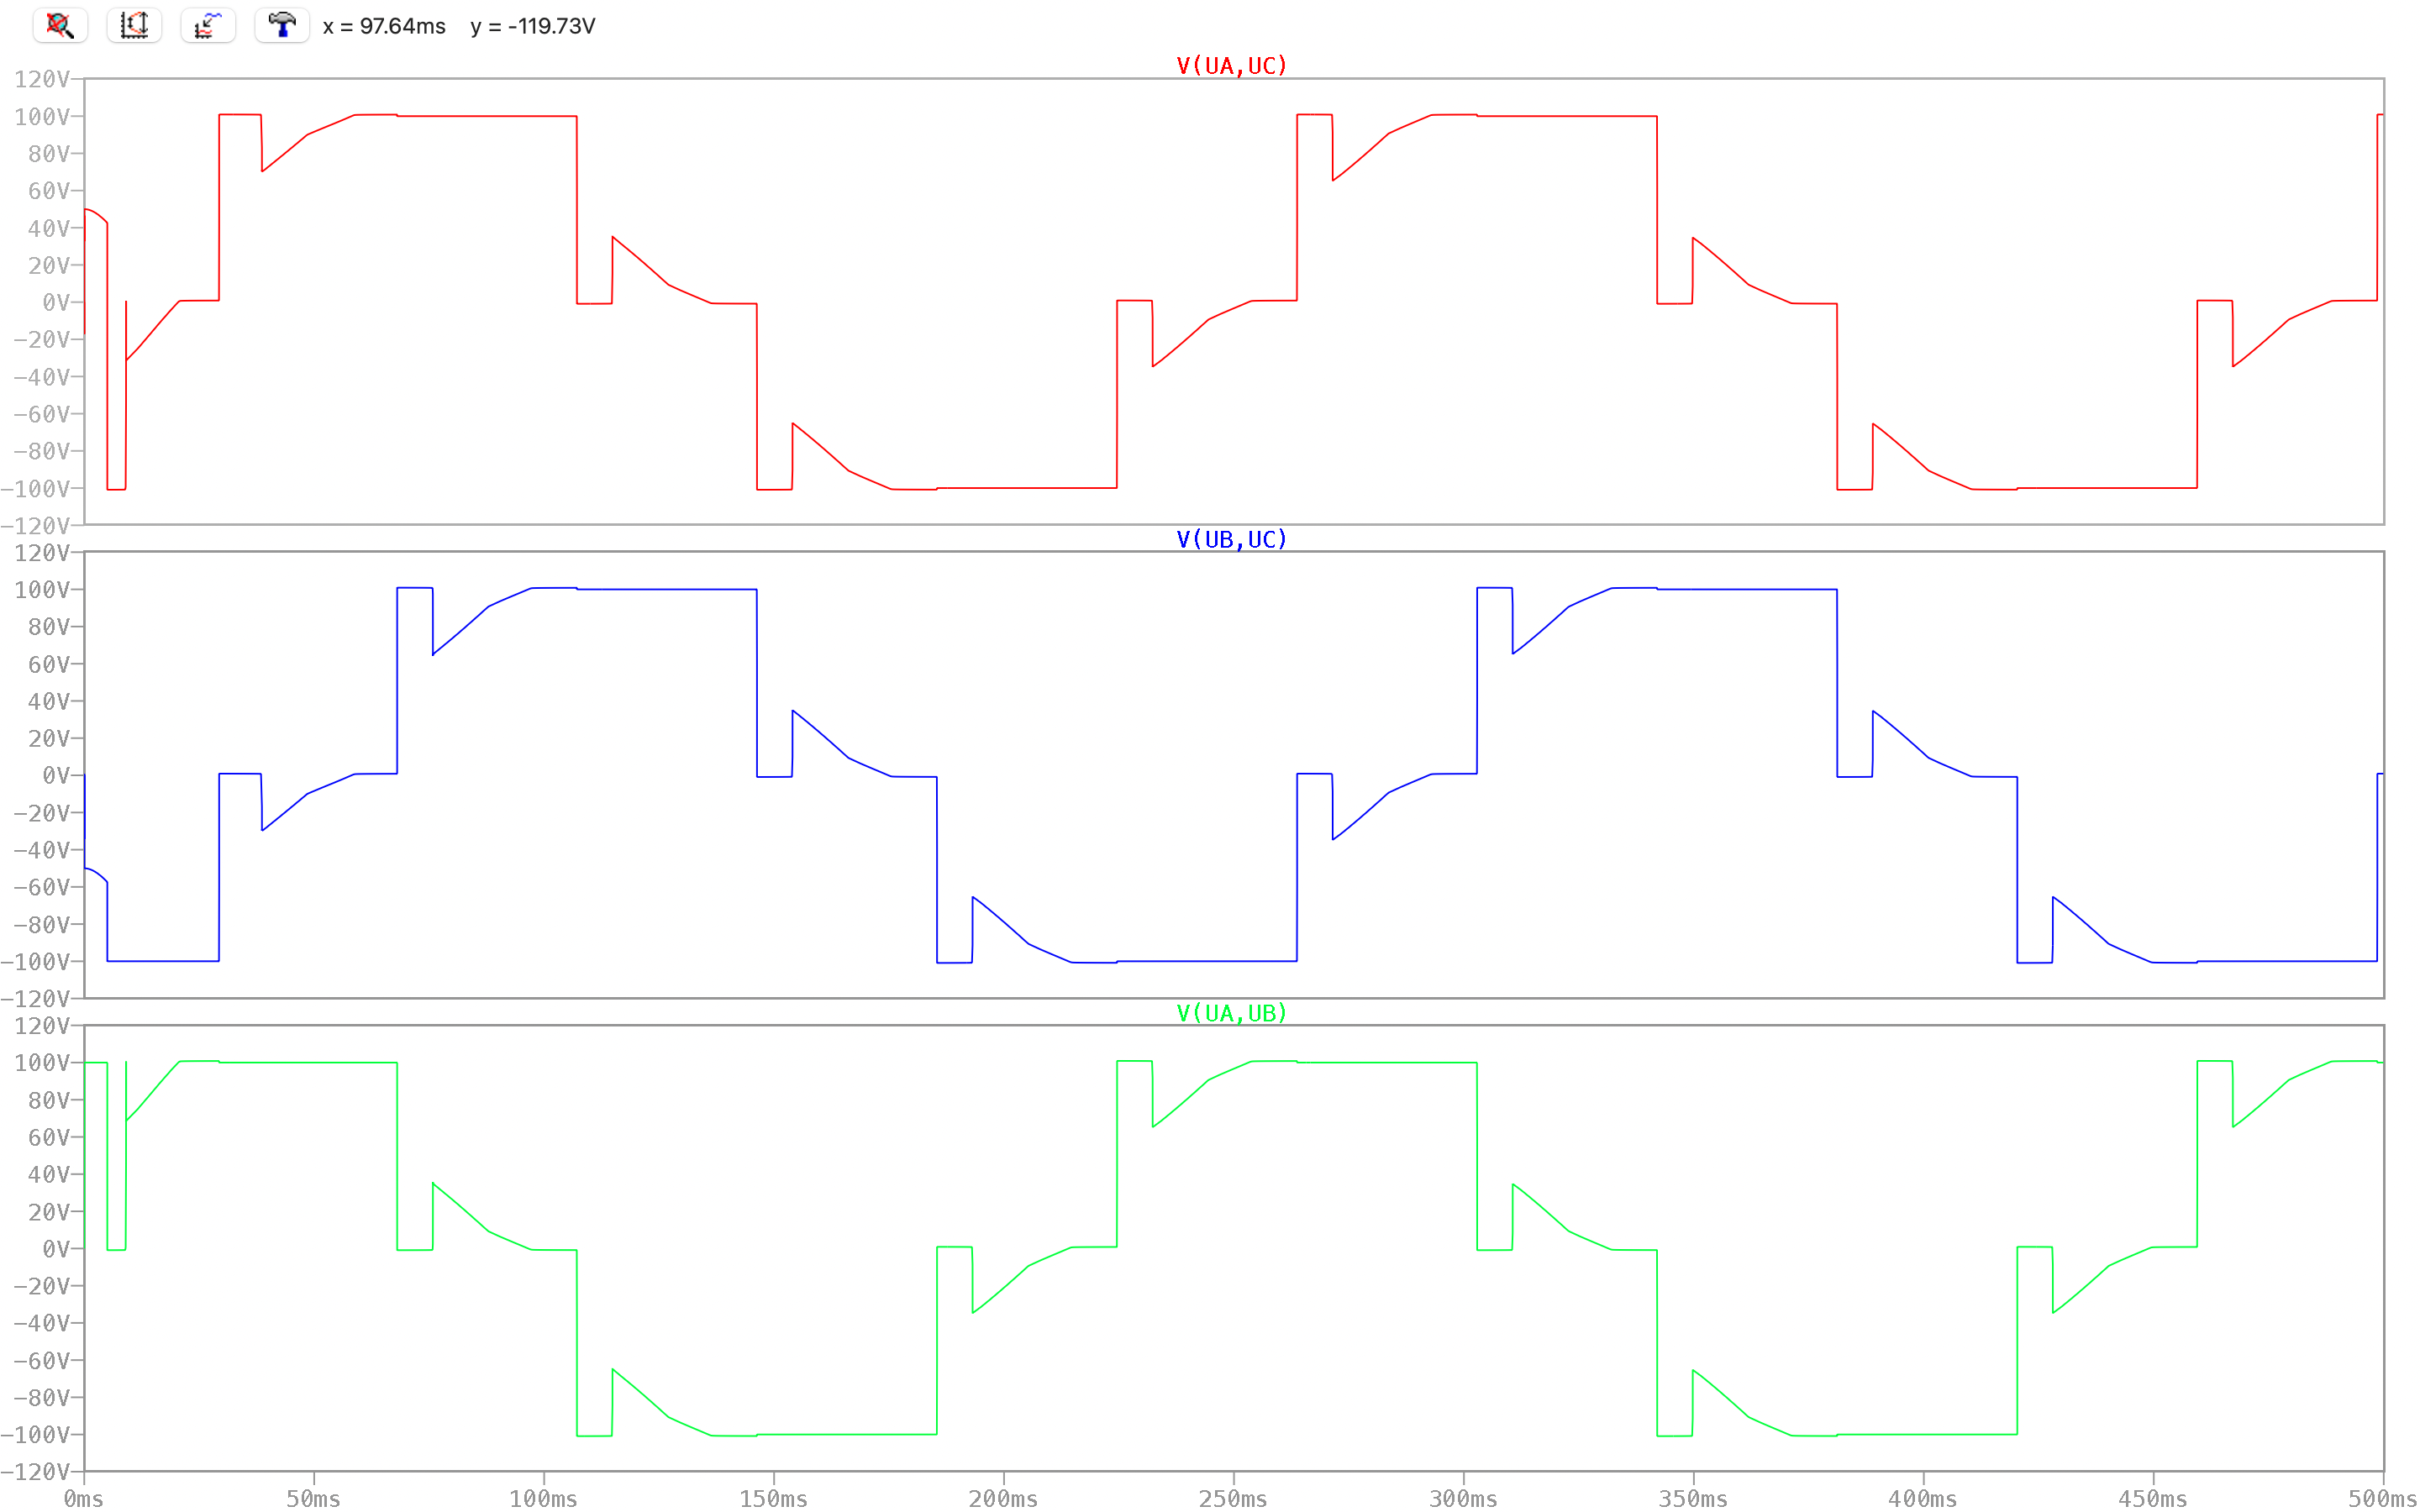
\includegraphics[width=0.8\textwidth]{images/napiecie_miedzyfazowe_bezczujnikowo.png}
    \caption{Wykresy napięć międzyfazowych dla sterowania bezczujnikowego $120^{\circ}$}
    \label{fig:120_napiecia_miedzyfazowe}
\end{figure}
Napięcia międzyfazowe przyjmują w tym typie sterowania kształt quasi-prostokątny. Skokowe zmiany wartości napięcia wynikają bezpośrednio z faktu dyskretnego przełączania tranzystorów co równe $60^{\circ}$ elektrycznych.

\begin{figure}[H]
    \centering
    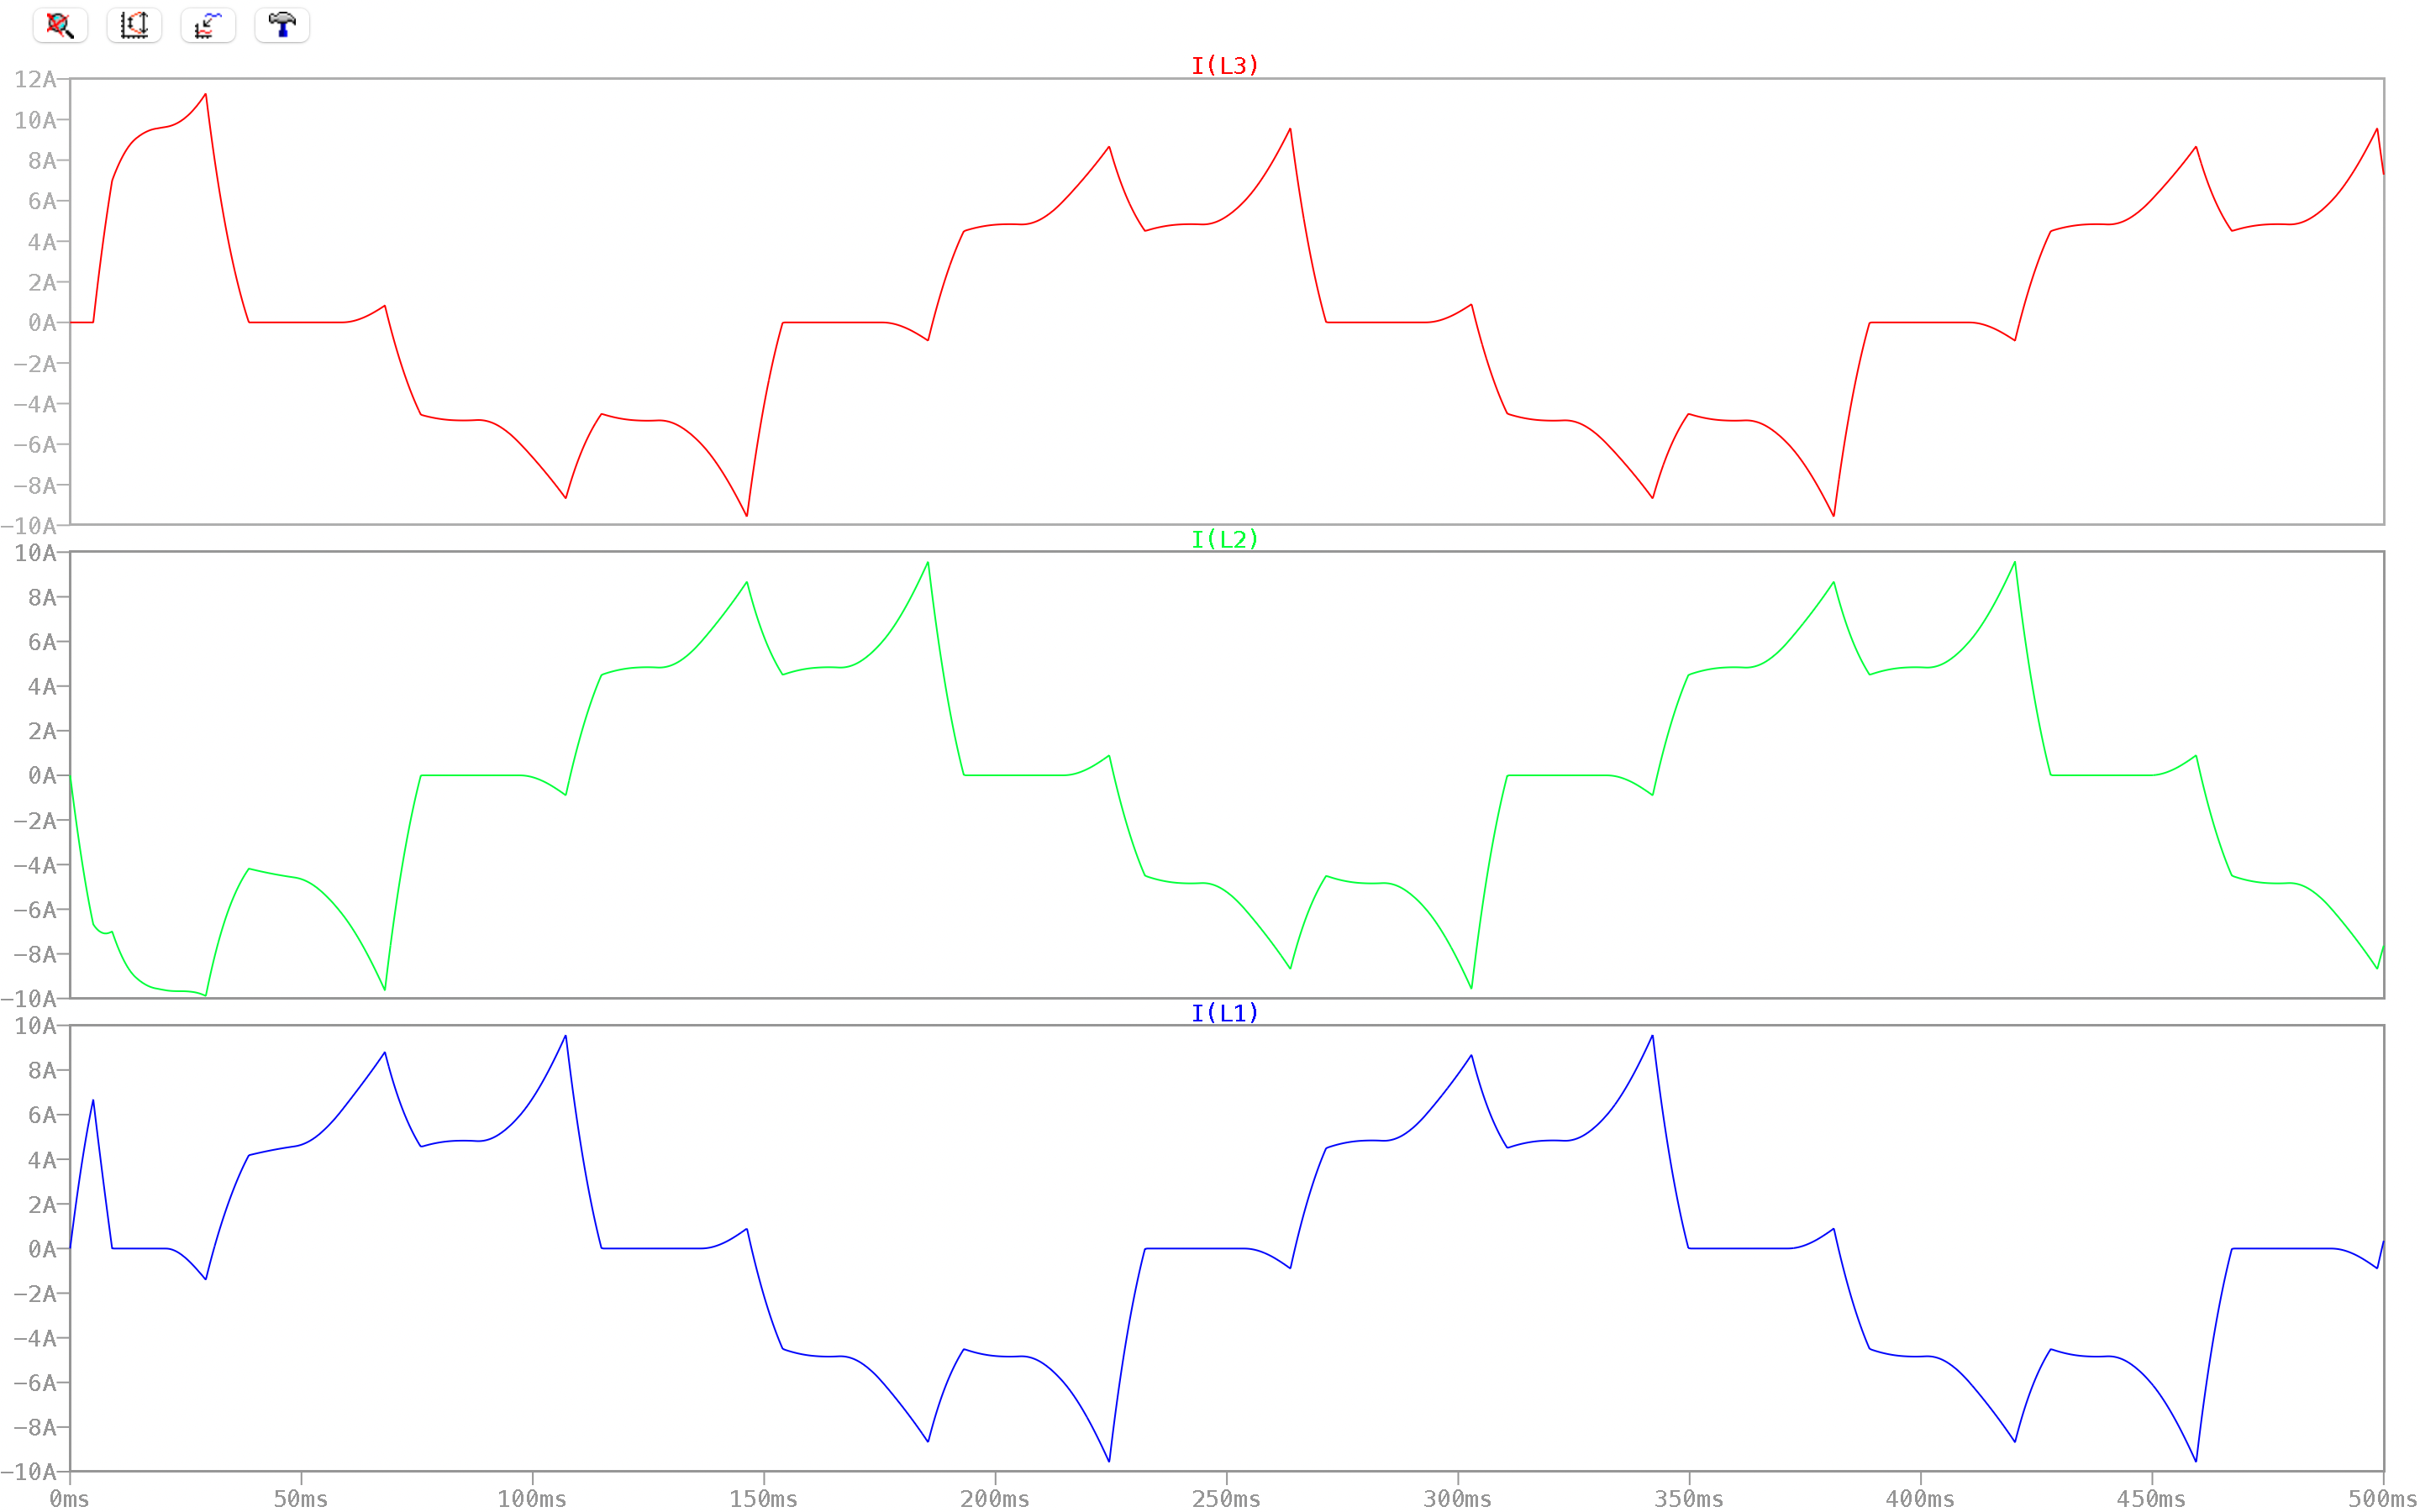
\includegraphics[width=0.8\textwidth]{images/prad_bezczujnikowo.png}
    \caption{Przebiegi prądów w poszczególnych fazach silnika ($120^{\circ}$ bezczujnikowo)}
    \label{fig:120_prady}
\end{figure}
Na wykresie prądów wyraźnie widoczne są $60^{\circ}$ okresy wyłączenia w każdej półfali. Zaobserwować można również charakterystyczne, ostre impulsy (tzw. szpilki) prądowe w momentach przełączania faz. Wynikają one z fizycznej indukcyjności uzwojeń (przeładowanie przez diody zwrotne) oraz faktu, że w zastosowanym uproszczonym algorytmie komutacja następuje bezpośrednio w momencie przejścia BEMF przez zero (w połowie okna komutacyjnego), co wymusza pewne przesunięcie fazowe względem idealnej komutacji czujnikowej.

\begin{figure}[H]
    \centering
    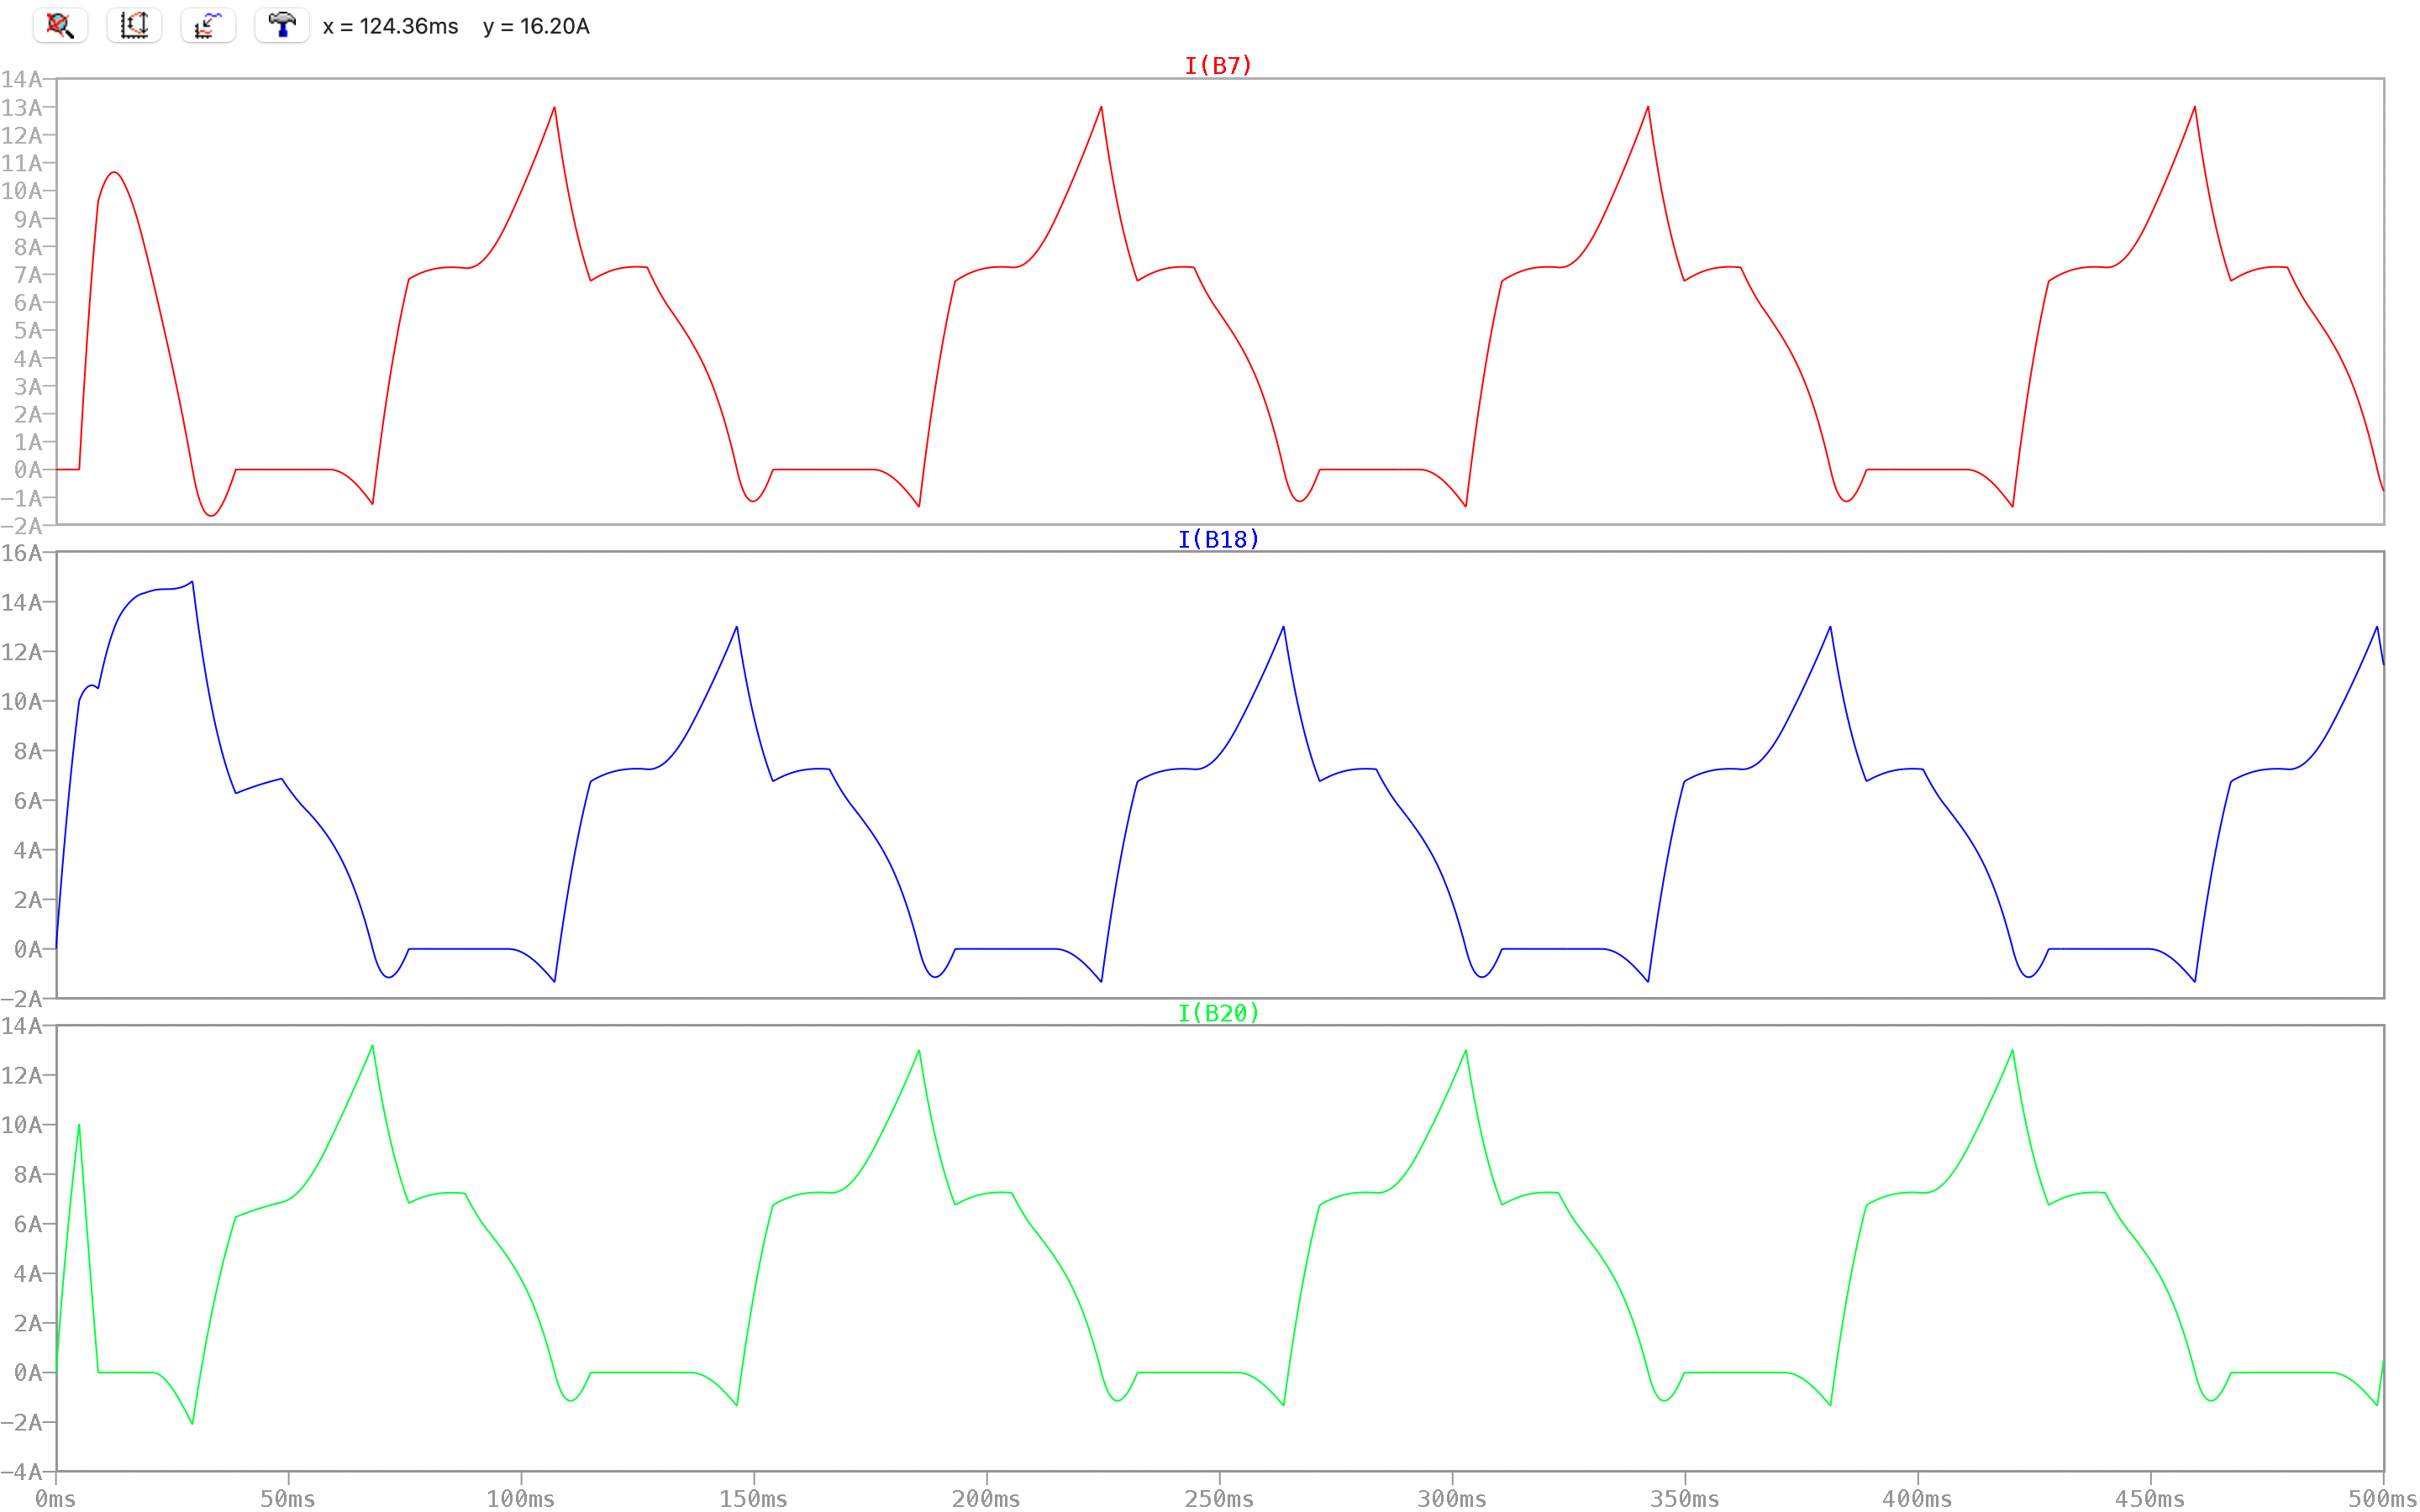
\includegraphics[width=0.8\textwidth]{images/moment_bezczujnikowo.png}
    \caption{Momenty poszczególnych faz silnika ($120^{\circ}$ bezczujnikowo)}
    \label{fig:120_momenty_fazowe}
\end{figure}
Poszczególne fazy maszyny generują moment obrotowy proporcjonalnie do płynącego przez nie prądu. Udział poszczególnych faz sumuje się, tworząc wspólną siłę napędową obracającą wirnik, jednak występują w nich zauważalne martwe strefy.

\begin{figure}[H]
    \centering
    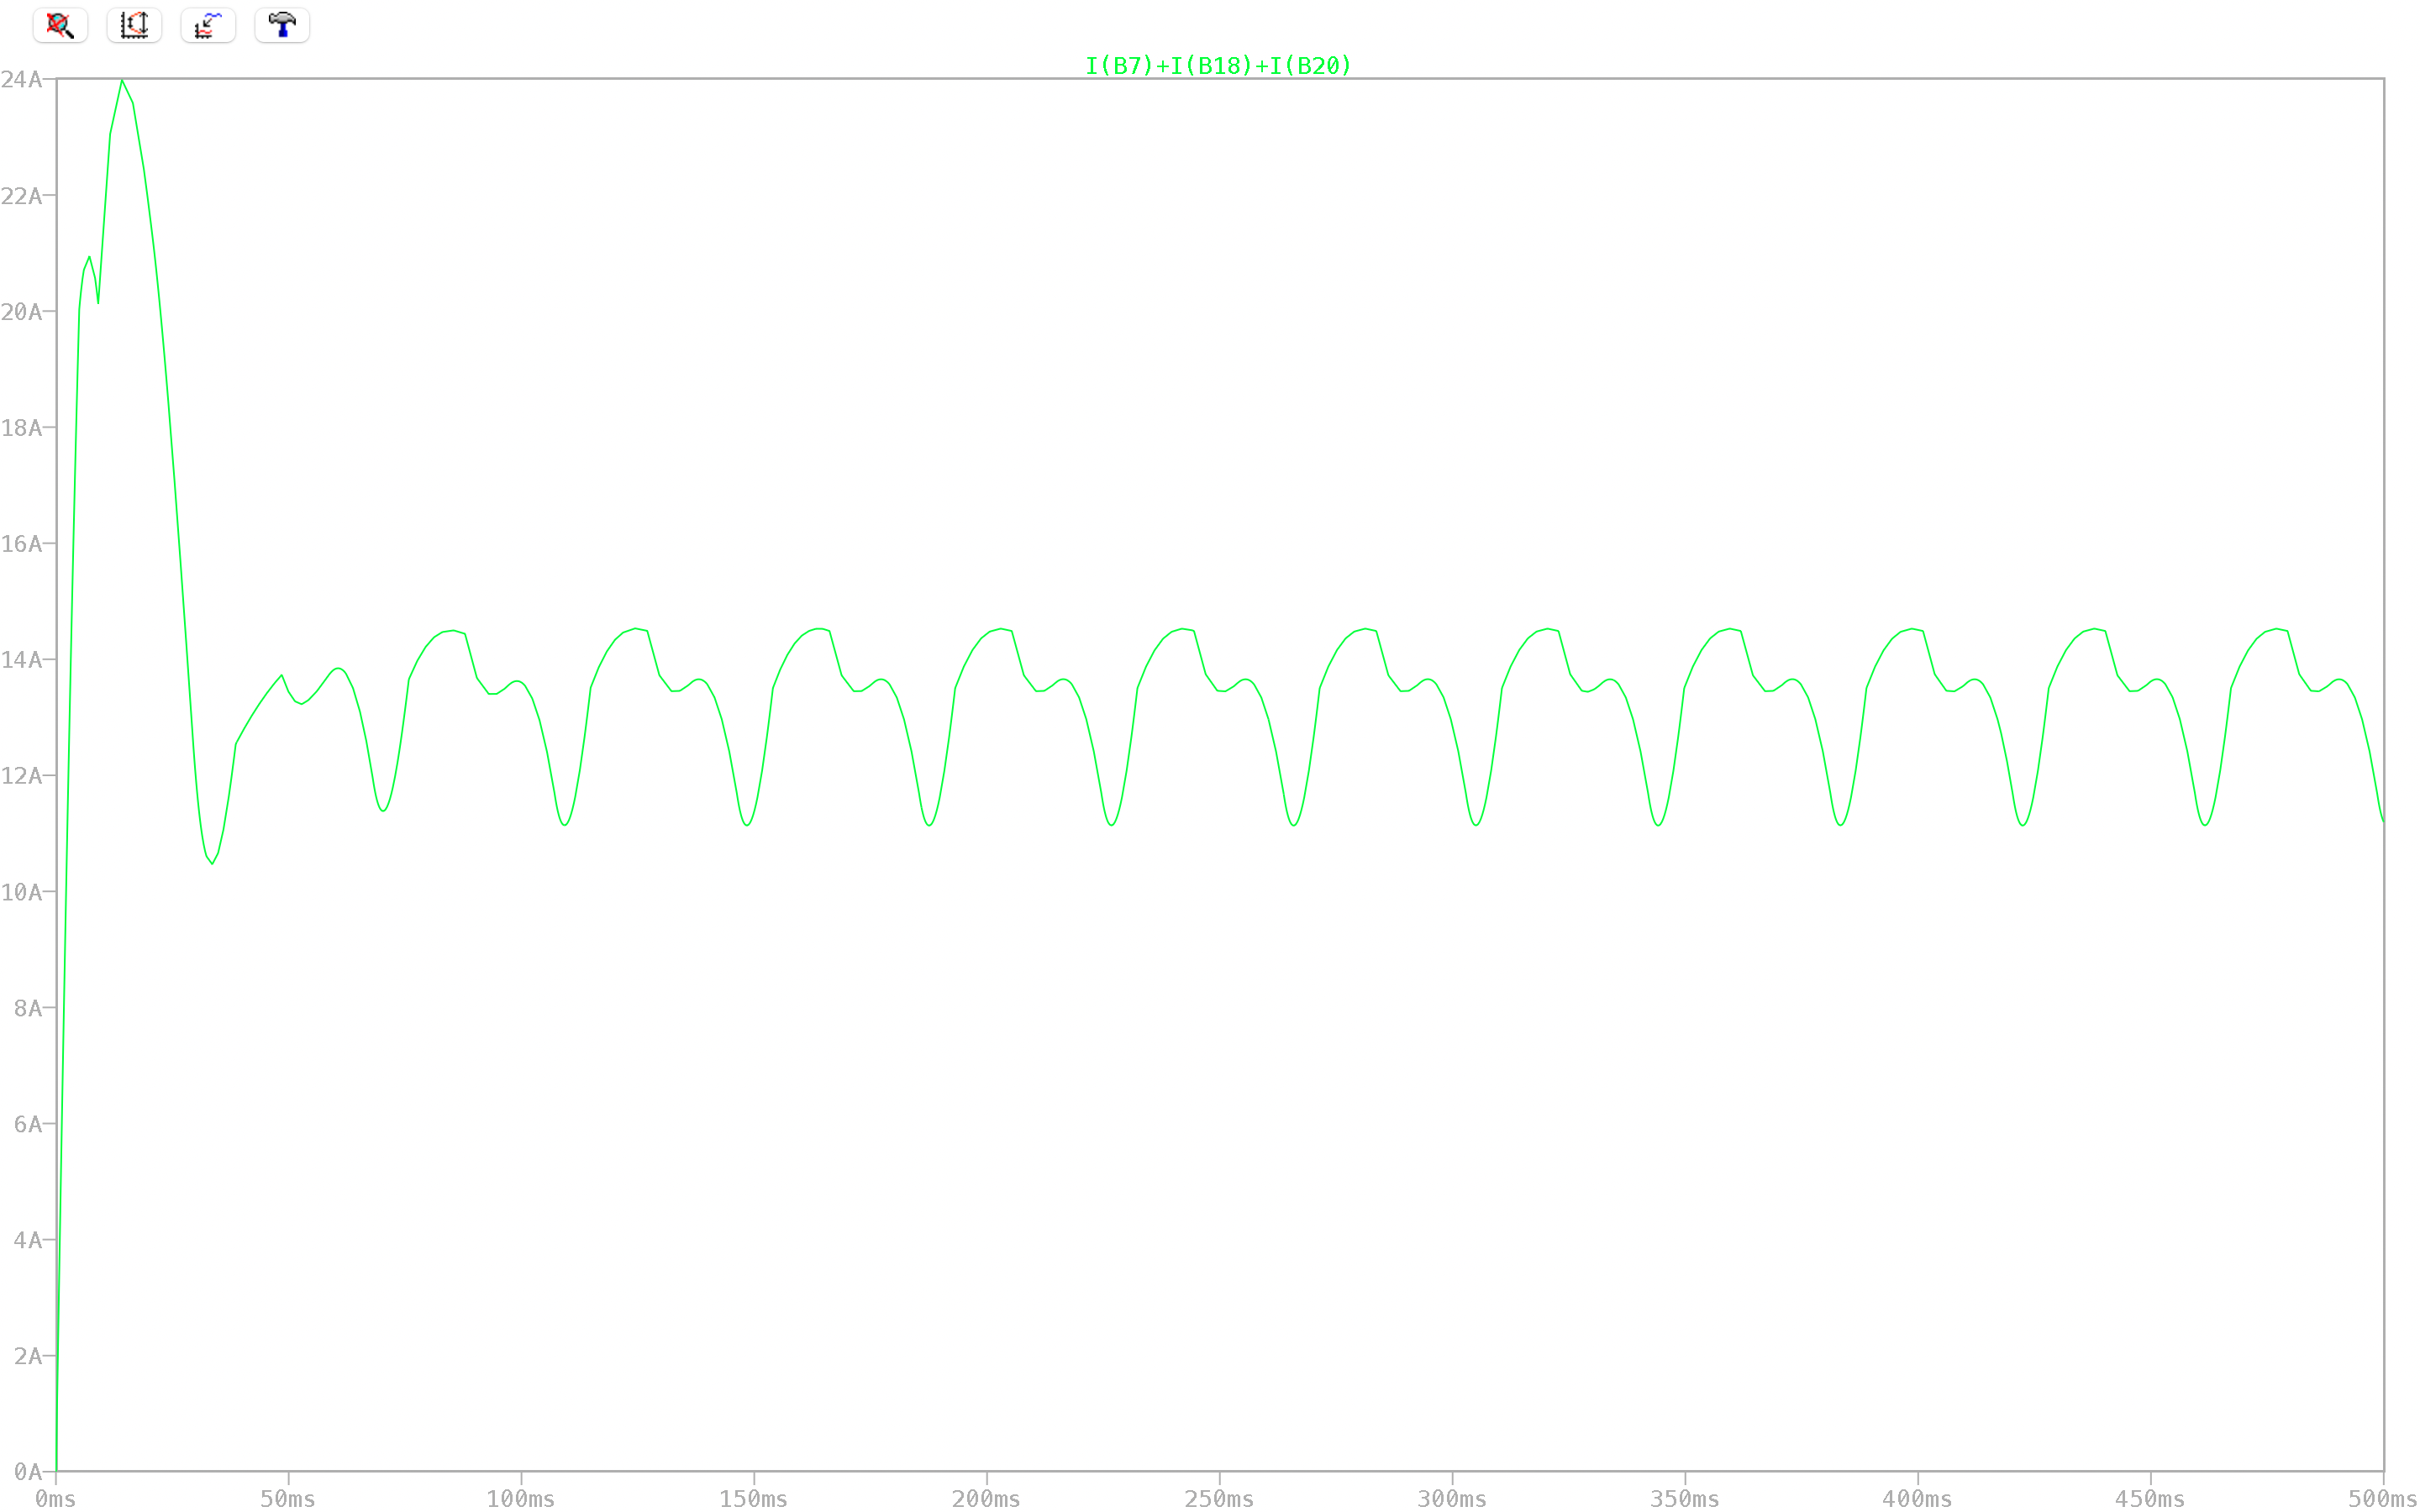
\includegraphics[width=0.8\textwidth]{images/moment_wspolny_bezczujnikowo.png}
    \caption{Całkowity moment elektromagnetyczny ($120^{\circ}$ bezczujnikowo)}
    \label{fig:120_moment_calkowity}
\end{figure}
Na przebiegu momentu całkowitego widoczne są charakterystyczne, głębokie zapady zwane tętnieniami komutacyjnymi (ang. torque ripple). Pojawiają się one dokładnie co $60^{\circ}$ w chwilach przełączania faz, co jest główną wadą metody sterowania opartej na prostokątnych sygnałach napięciowych.

\begin{figure}[H]
    \centering
    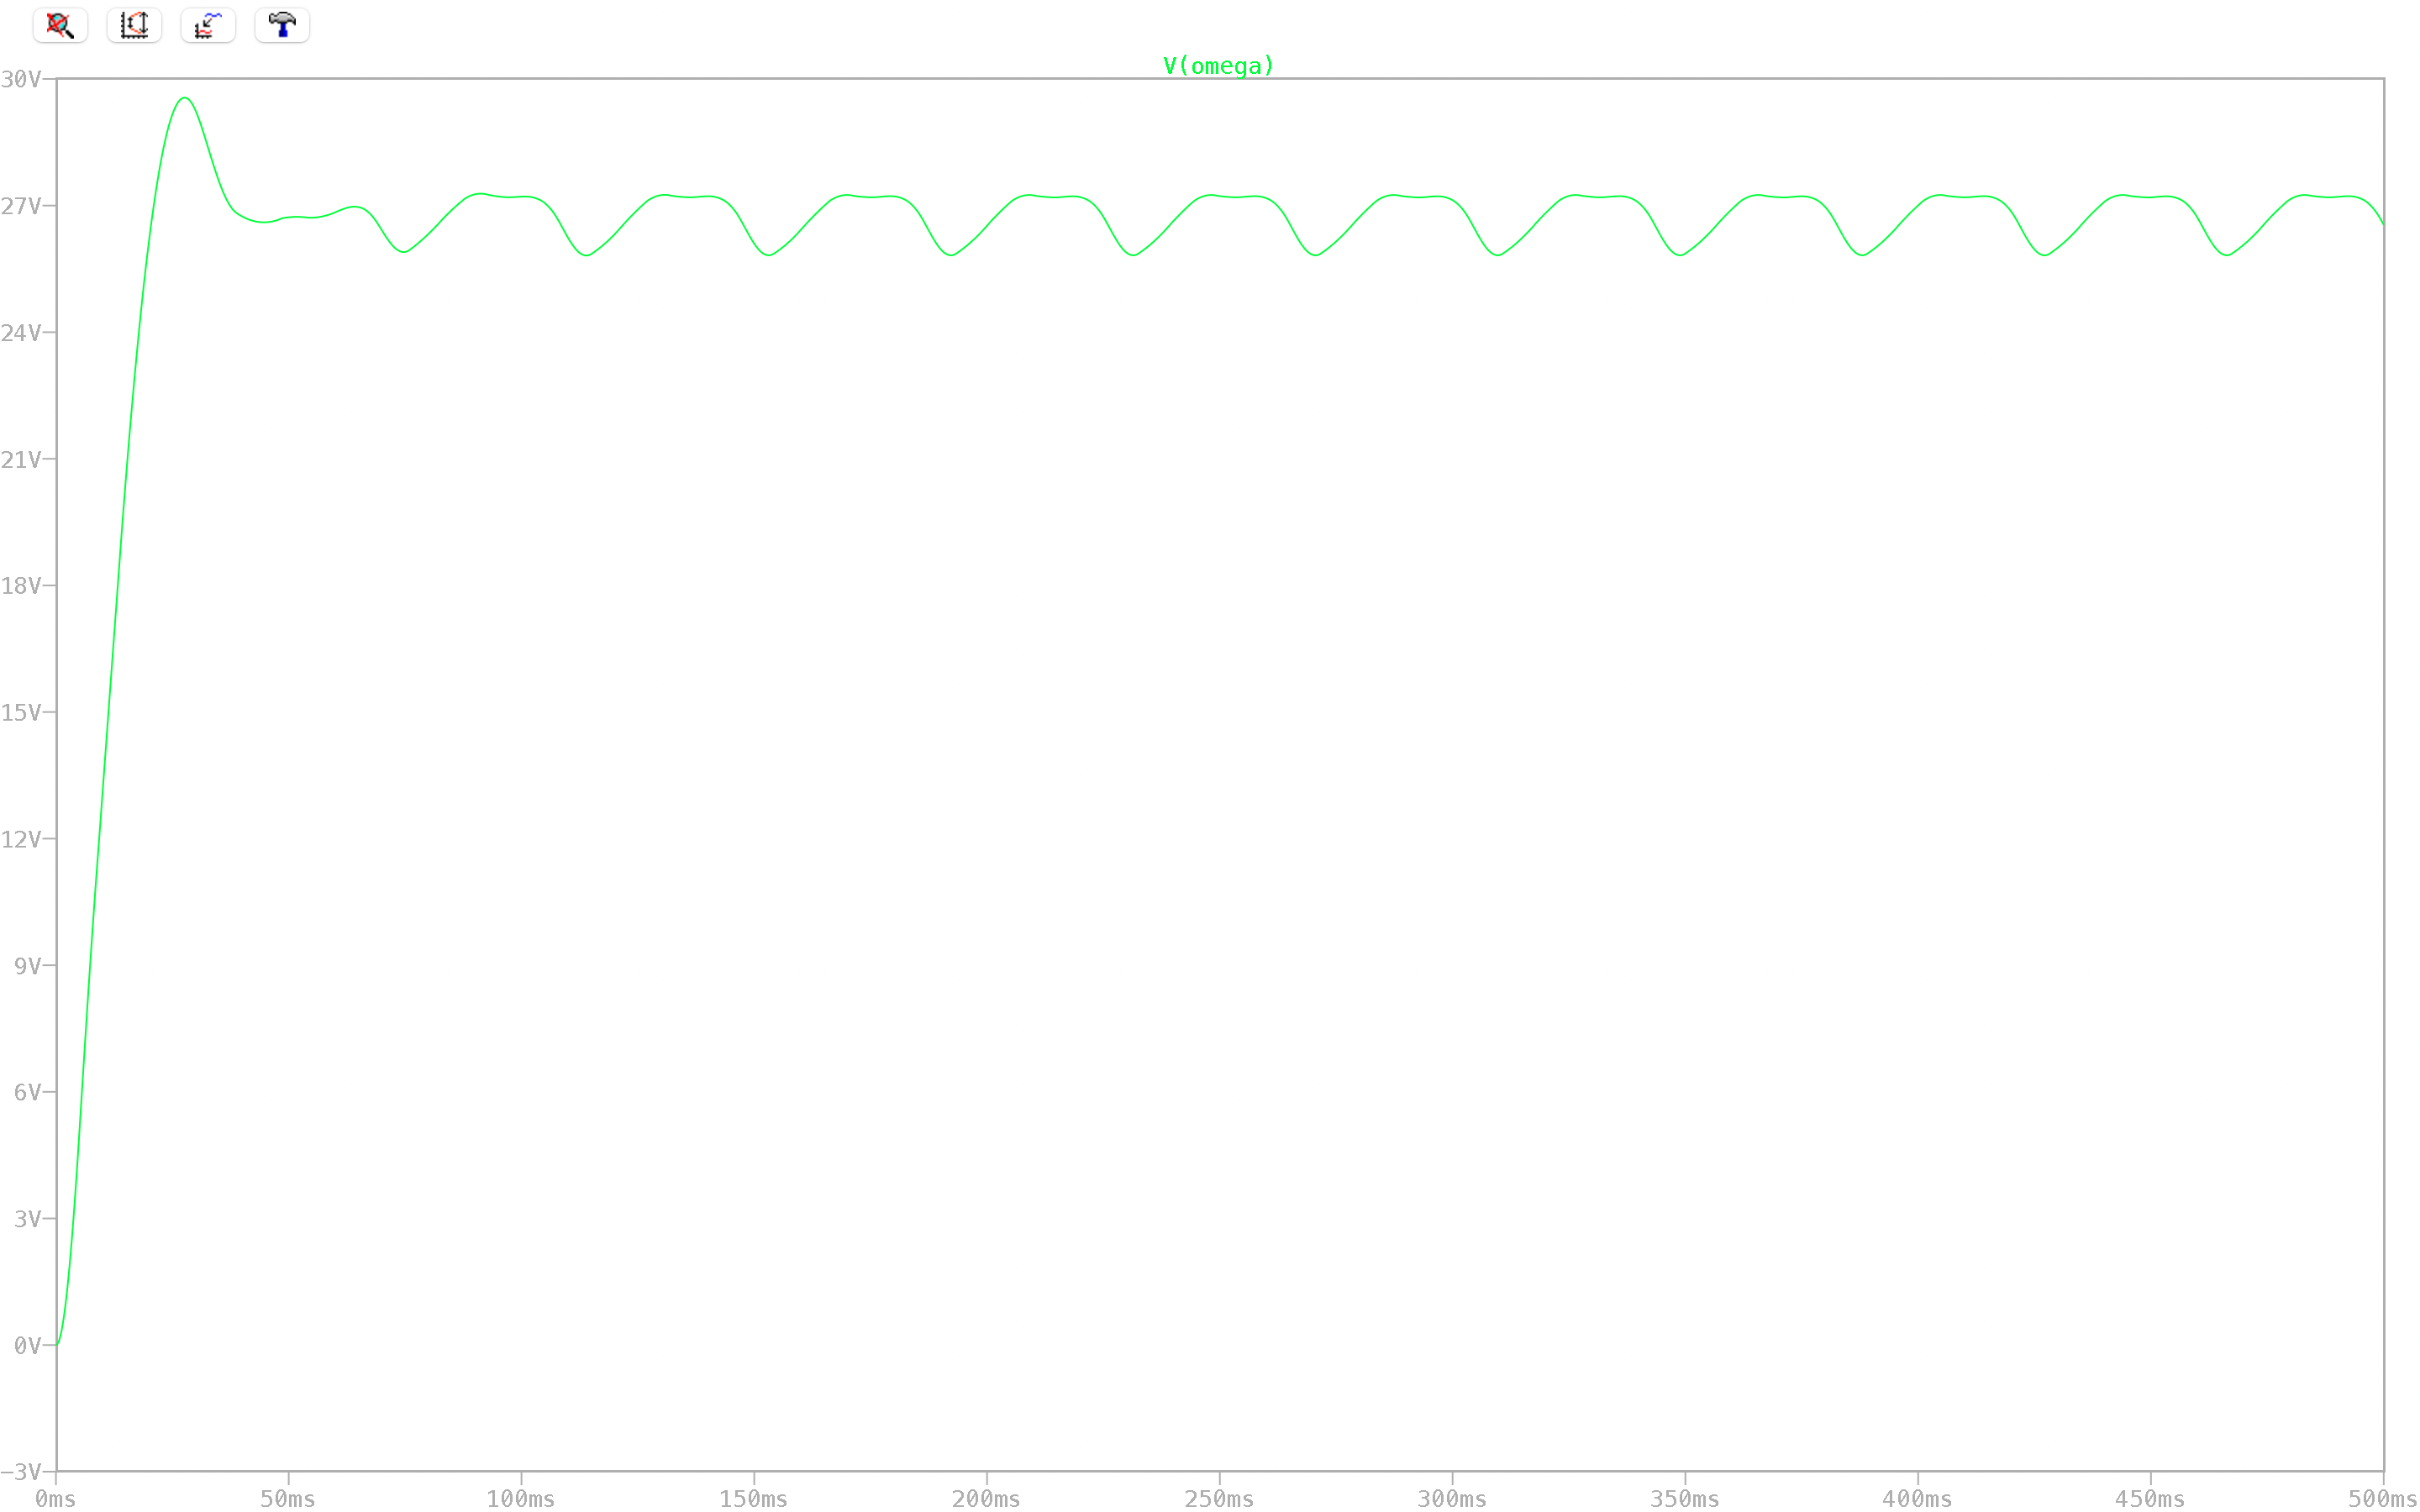
\includegraphics[width=0.8\textwidth]{images/omega_bezczujnikowo.png}
    \caption{Przebieg prędkości kątowej silnika ($120^{\circ}$ bezczujnikowo)}
    \label{fig:120_predkosc}
\end{figure}
Po fazie rozruchu i przekroczeniu prędkości bazowej (\texttt{omega\_min}), system precyzyjnie śledzi indukowaną siłę elektromotoryczną. Silne tętnienia momentu wywołują jednak drobne oscylacje prędkości obrotowej w stanie ustalonym, co w warunkach fizycznych obniża kulturę pracy napędu.


\subsection{Sterowanie trapezowe przy kącie załączania fazy rozszerzonym o 150 stopni elektrycznych}

Metoda sterowania rozszerzonego polega na sztucznym wydłużeniu czasu przewodzenia
każdego z sześciu tranzystorów mostka falownika z klasycznych $120^{\circ}$ do $150^{\circ}$ elektrycznych. 
Efektem tego zabiegu jest skrócenie czasu, w którym dana faza pozostaje odłączona od zasilania (z $60^{\circ}$ 
do zaledwie $30^{\circ}$). Taki sposób komutacji pozwala na to, aby przez krótkie okresy ($30^{\circ}$) prąd 
przewodziły wszystkie trzy fazy jednocześnie. Umożliwia to znacznie łagodniejsze przejmowanie prądu, co w bezpośredni
sposób przekłada się na redukcję szarpnięć momentu elektromagnetycznego i poprawia płynność oraz kulturę pracy napędu.

Implementacja tej metody w środowisku LTspice wymagała modyfikacji sygnałów wyzwalających bramki tranzystorów.
Dokonano tego poprzez dodanie opóźnienia do sygnałów bazowych, co pozwoliło na przedłużenie każdego impulsu dokładnie 
o $30^{\circ}$ elektrycznych. Zestawienie zmodyfikowanych równań dla modelu umieszczono w Tabeli 2.

\begin{table}[H]
\centering
\renewcommand{\arraystretch}{1.6}
\small
\begin{tabular}{|c|m{13.5cm}|}
\hline
\rowcolor{gray!20}
\textbf{Klucz} & \textbf{Zdefiniowany sygnał sterujący (Równanie LTspice)} \\
\hline
$K_1$ (Górny U) & \texttt{V=if( (V(H1)>0 \& V(H3)<1) | delay(V(H1)>0 \& V(H3)<1, pi/(6*V(omega))), 1, 0 )} \\
\hline
$K_4$ (Dolny U) & \texttt{V=if( (V(H1)<1 \& V(H3)>0) | delay(V(H1)<1 \& V(H3)>0, pi/(6*V(omega))), 1, 0 )} \\
\hline
$K_3$ (Górny V) & \texttt{V=if( (V(H2)>0 \& V(H1)<1) | delay(V(H2)>0 \& V(H1)<1, pi/(6*V(omega))), 1, 0 )} \\
\hline
$K_6$ (Dolny V) & \texttt{V=if( (V(H2)<1 \& V(H1)>0) | delay(V(H2)<1 \& V(H1)>0, pi/(6*V(omega))), 1, 0 )} \\
\hline
$K_5$ (Górny W) & \texttt{V=if( (V(H3)>0 \& V(H2)<1) | delay(V(H3)>0 \& V(H2)<1, pi/(6*V(omega))), 1, 0 )} \\
\hline
$K_2$ (Dolny W) & \texttt{V=if( (V(H3)<1 \& V(H2)>0) | delay(V(H3)<1 \& V(H2)>0, pi/(6*V(omega))), 1, 0 )} \\
\hline
\end{tabular}
\caption{Definicja zmodyfikowanych sygnałów sterujących dla metody $150^{\circ}$.}
\label{tab:klucze_150}
\end{table}

Podstawowy warunek przewodzenia został tu zsumowany logicznie ze swoją własną, opóźnioną kopią. Zastosowane równanie dynamicznie wylicza opóźnienie, dzieląc wartość kąta $\pi/6$ ($30^{\circ}$) przez aktualną prędkość silnika. Poniżej zamieszczono przebiegi ilustrujące działanie tego rozwiązania.

\begin{figure}[H]
    \centering
    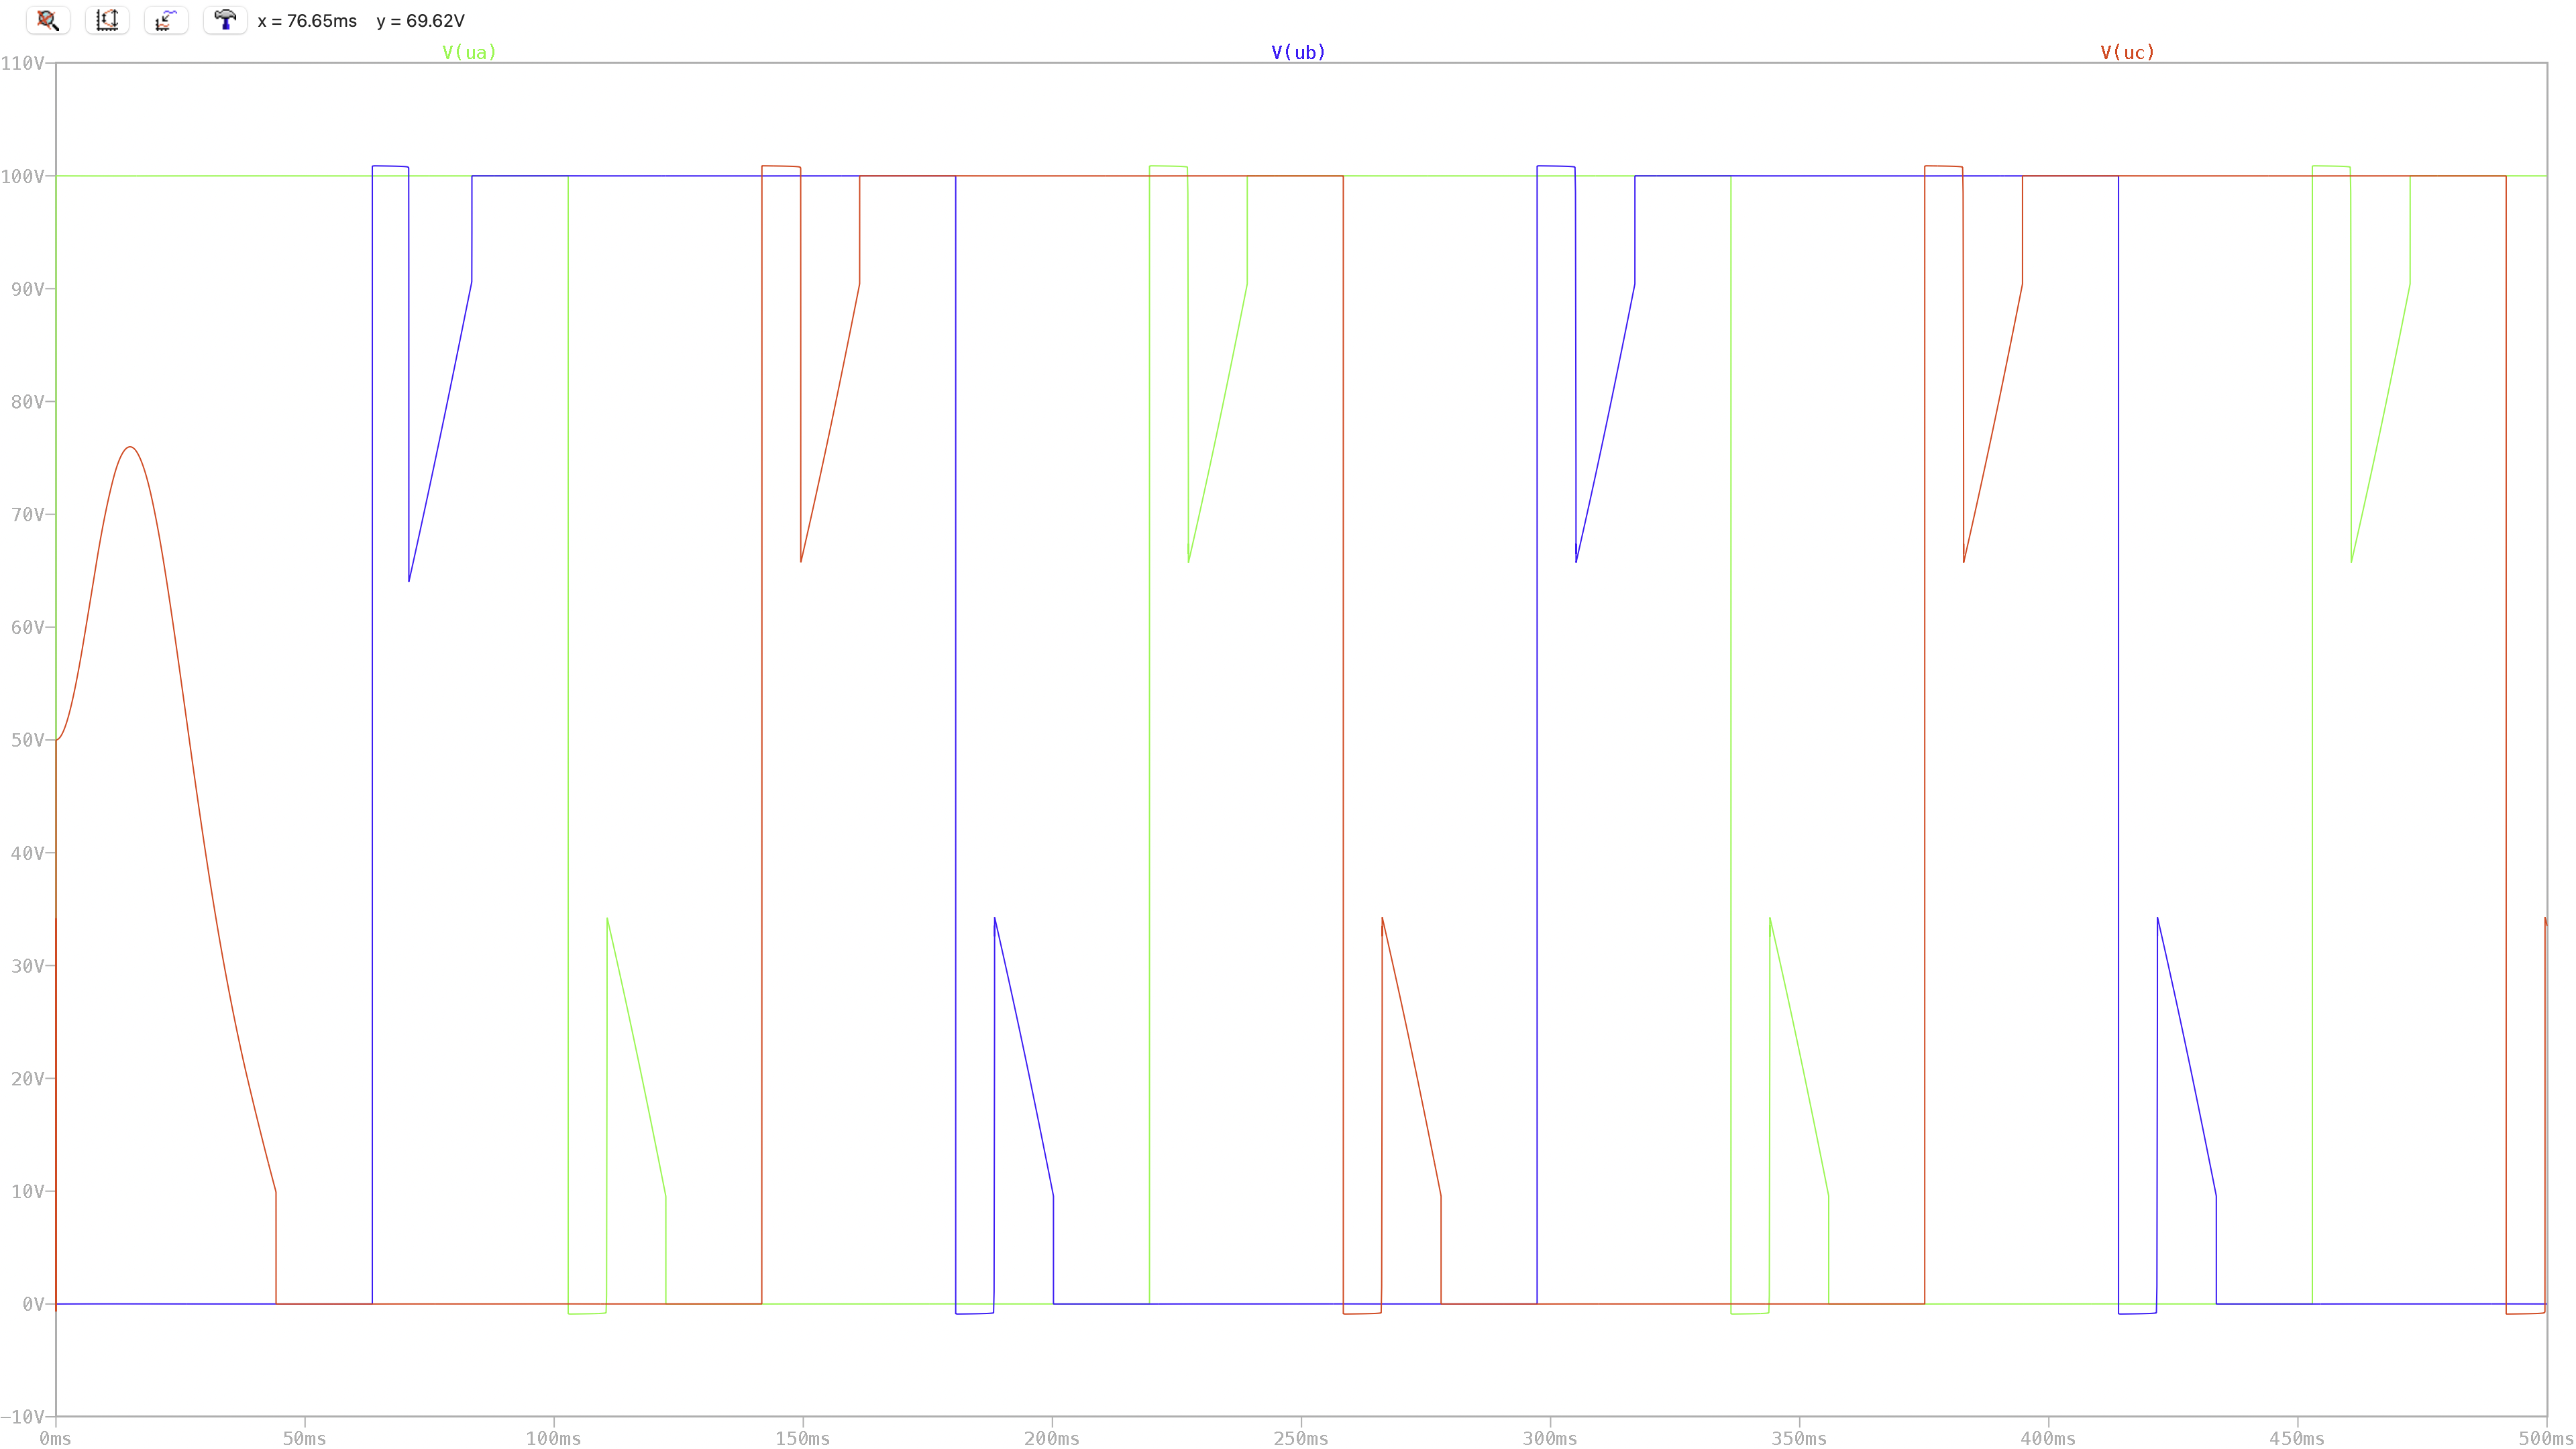
\includegraphics[width=0.8\textwidth]{images/fazowe_150.png}
    \caption{Wykresy napięć fazowych dla sterowania $150^{\circ}$}
    \label{fig:150_napiecia_fazowe}
\end{figure}
Wskutek wydłużenia czasu załączenia kluczy zredukowano przerwy w zasilaniu. Obszary, w których faza wisi w powietrzu, uległy znacznemu zwężeniu do $30^{\circ}$, co upodabnia kształt krzywej napięcia do łagodniejszego, ciągłego przebiegu.

\begin{figure}[H]
    \centering
    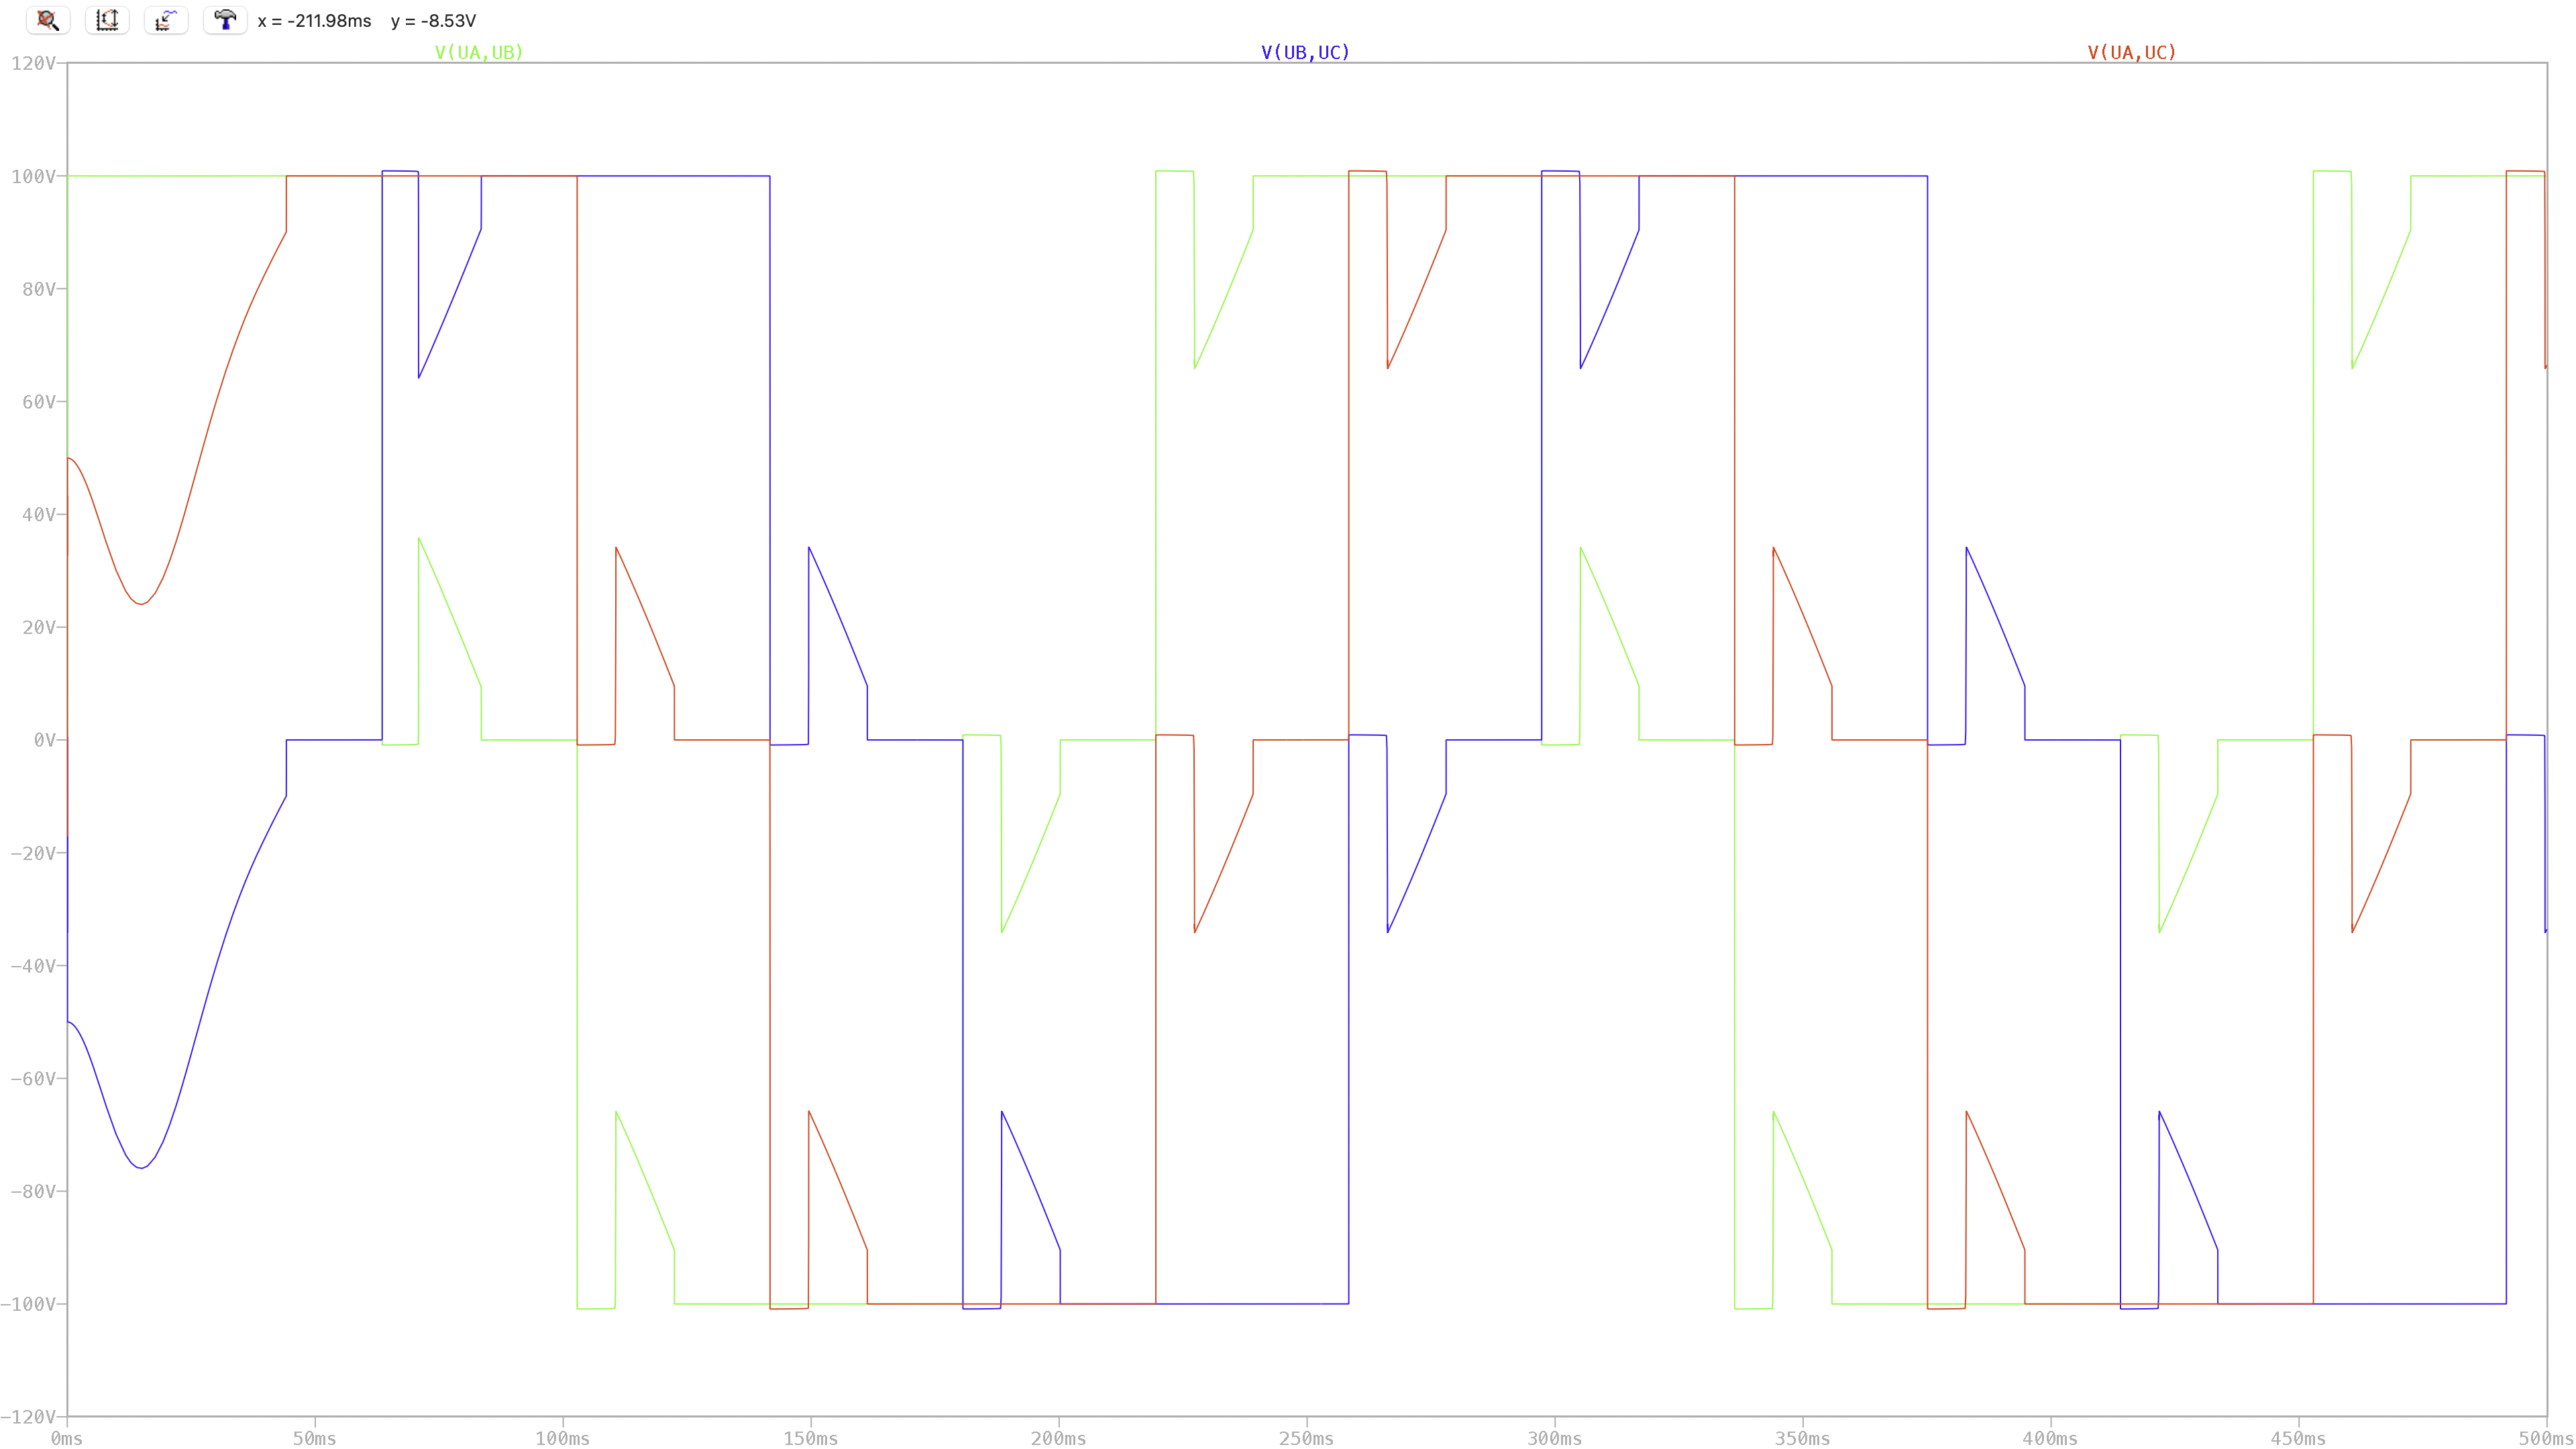
\includegraphics[width=0.8\textwidth]{images/miedzyfazowe150.png}
    \caption{Wykresy napięć międzyfazowych dla sterowania $150^{\circ}$}
    \label{fig:150_napiecia_miedzyfazowe}
\end{figure}
Napięcia występujące pomiędzy fazami stają się szersze i przyjmują nieco inny kształt. Zjawisko to bezpośrednio wiąże się z etapami jednoczesnego przewodzenia prądu w trzech fazach podczas przedłużonych cykli komutacji.

\begin{figure}[H]
    \centering
    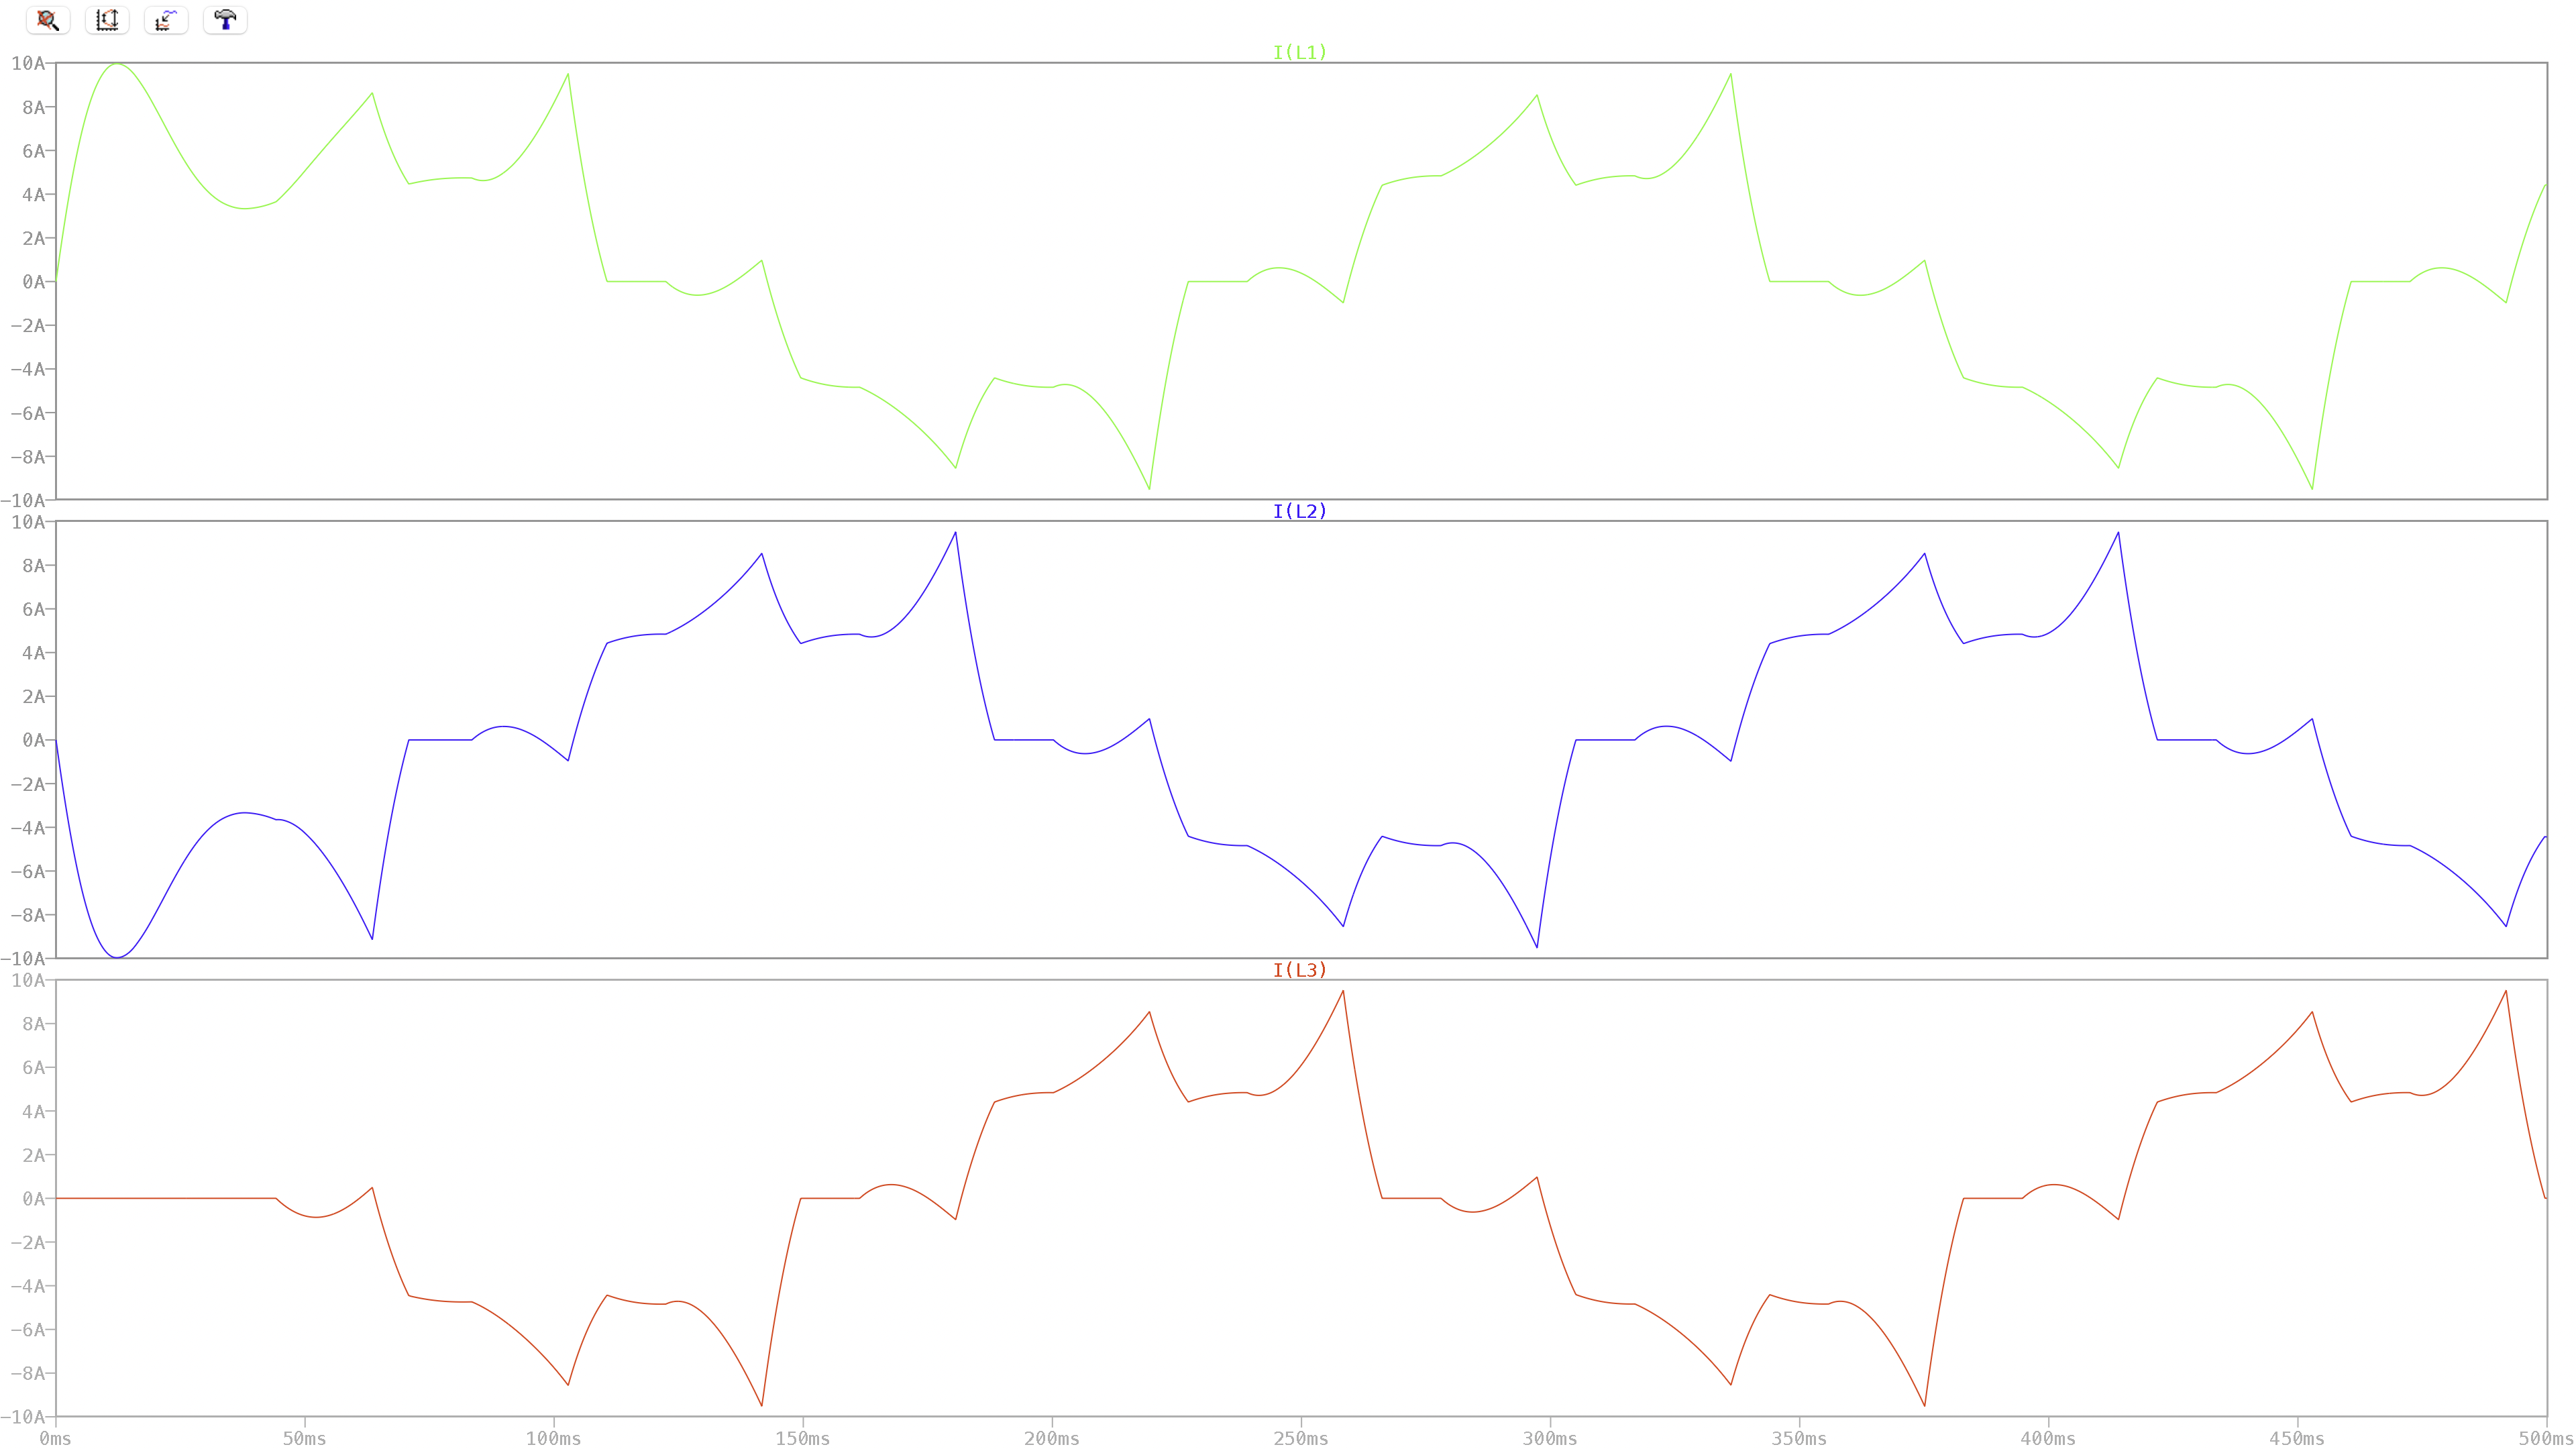
\includegraphics[width=0.8\textwidth]{images/prady_150.png}
    \caption{Przebiegi prądów fazowych ($150^{\circ}$)}
    \label{fig:150_prady}
\end{figure}
Na wykresie prądowym widać znaczne ograniczenie przerw beznapięciowych, które zmalały do krótkich odcinków $30$-stopniowych. Skutkuje to dużo płynniejszym narastaniem oraz opadaniem natężenia prądu, chroniąc układ przed obciążeniami dynamicznymi.

\begin{figure}[H]
    \centering
    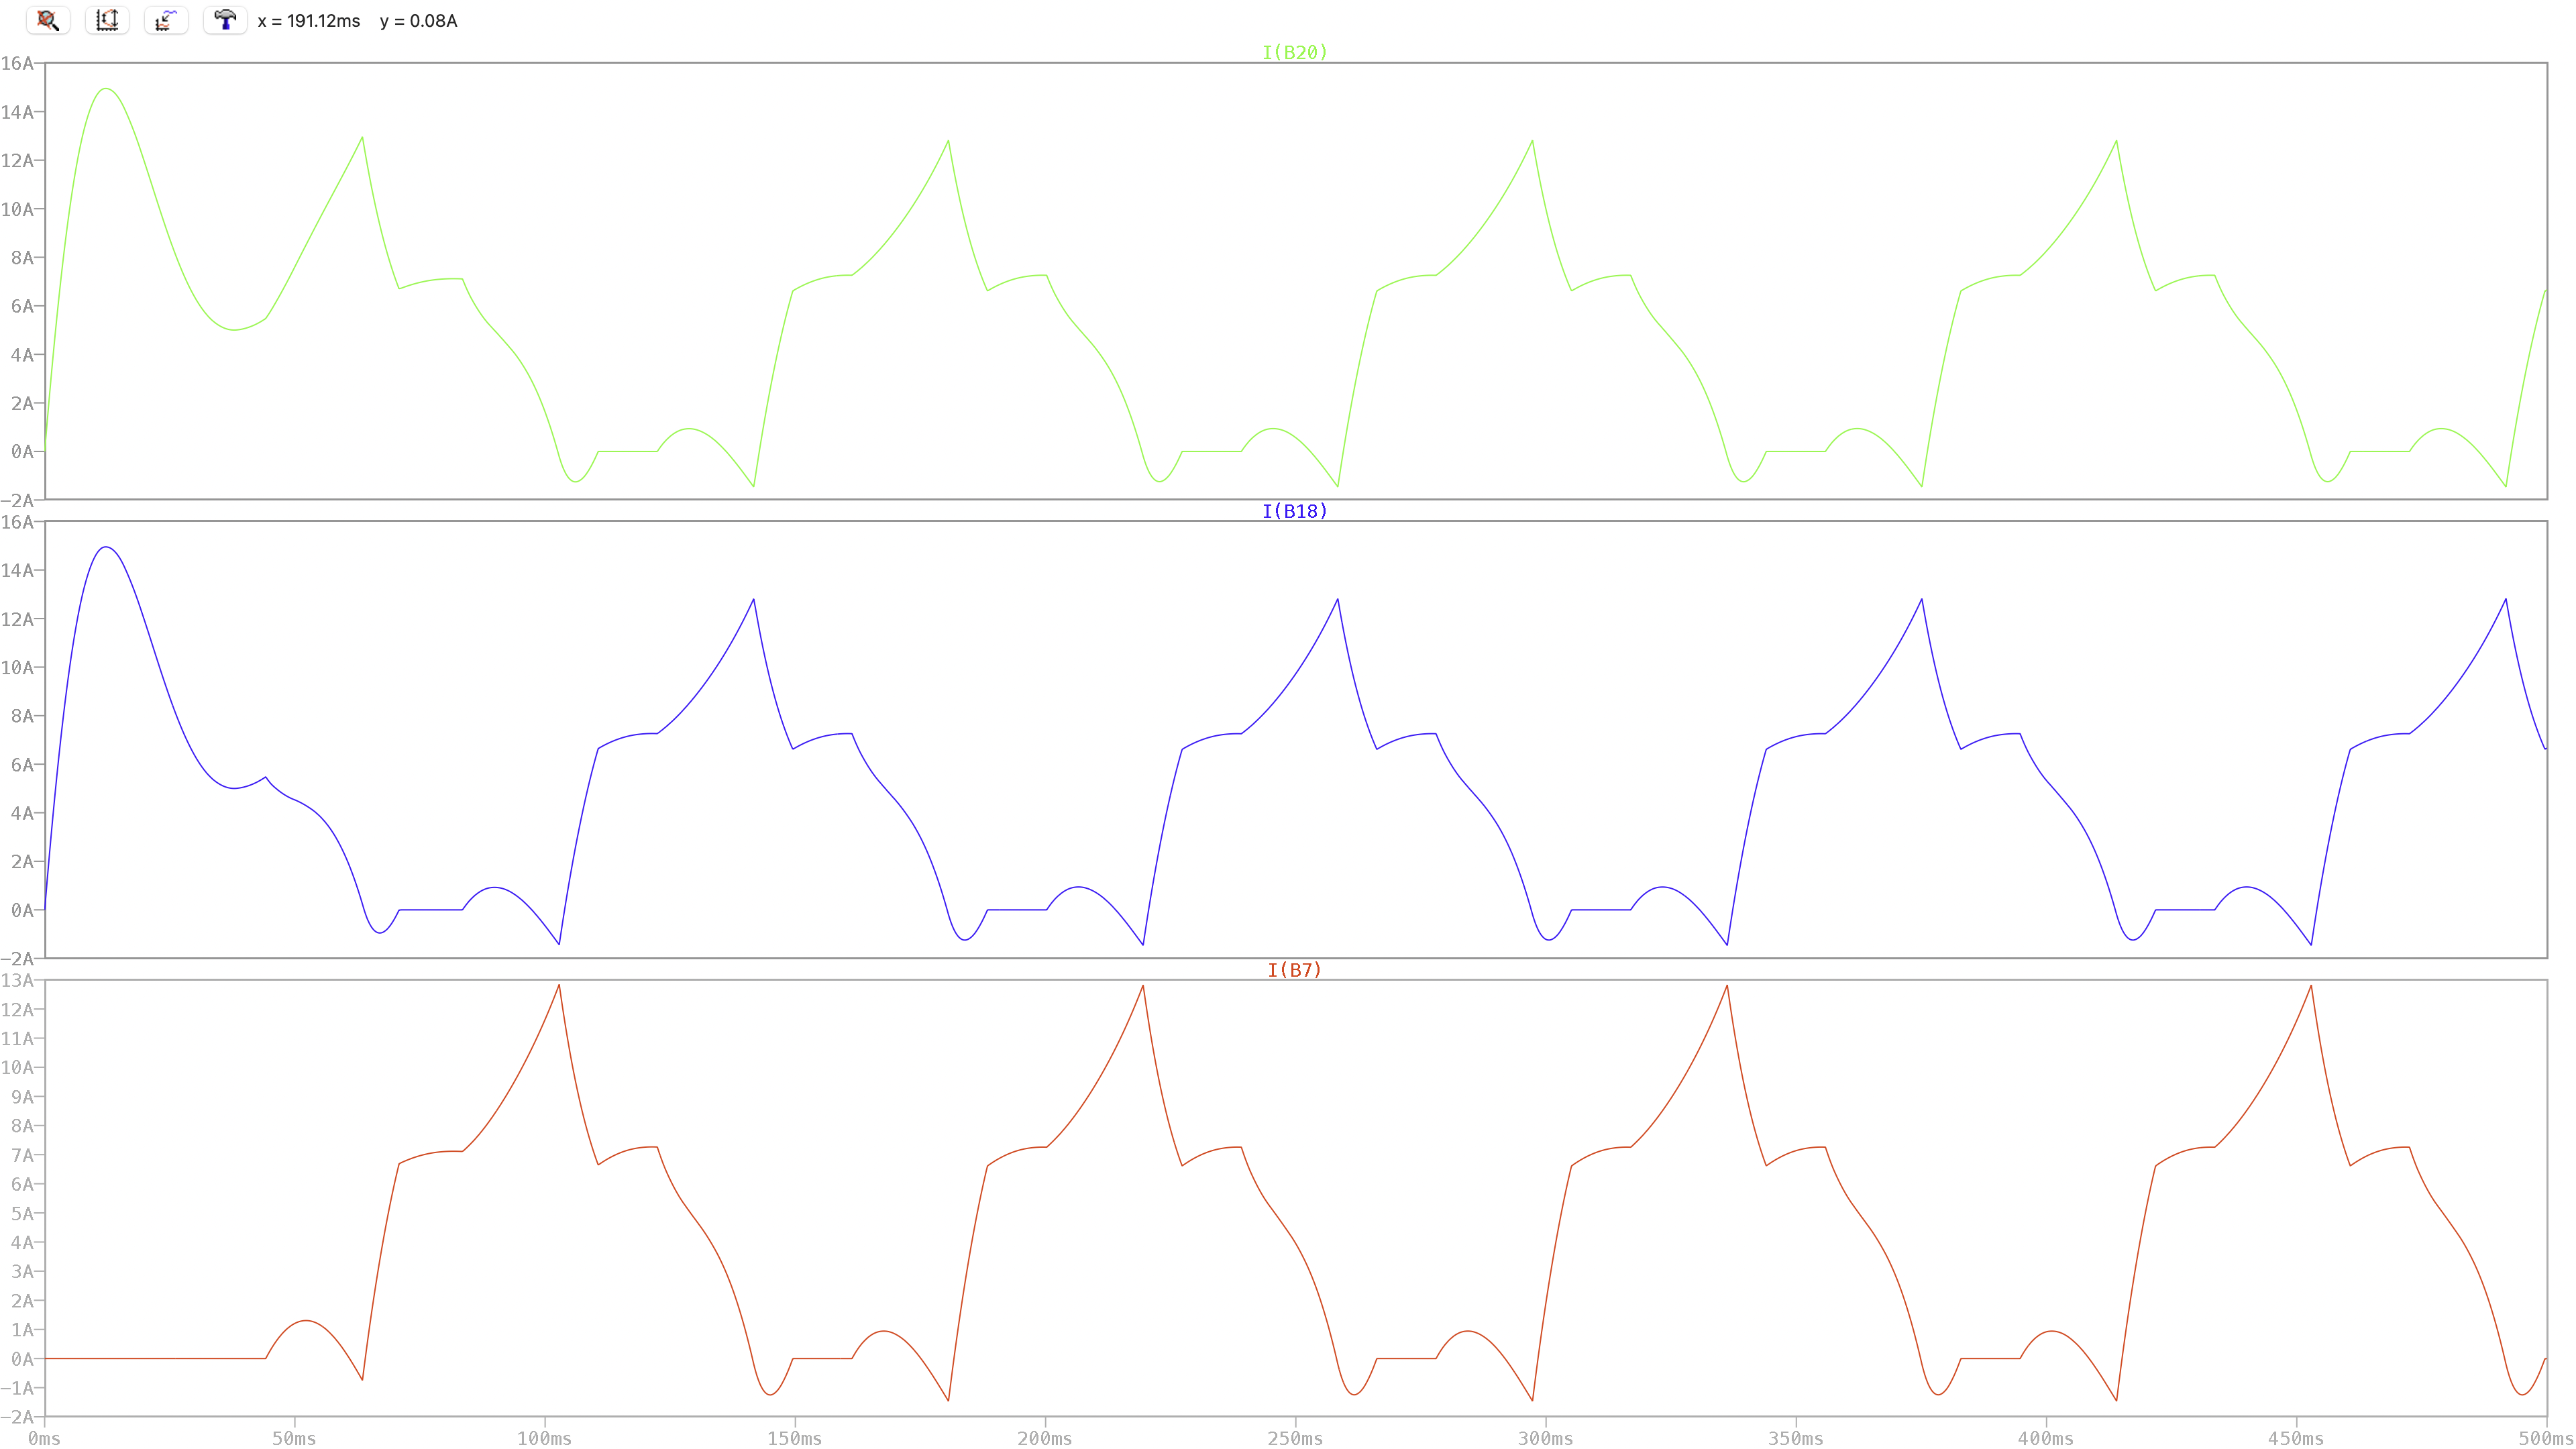
\includegraphics[width=0.8\textwidth]{images/momenty_150.png}
    \caption{Momenty fazowe oraz całkowity moment elektromagnetyczny ($150^{\circ}$)}
    \label{fig:150_momenty}
\end{figure}
Całkowity moment wypadkowy maszyny charakteryzuje się zdecydowanie spłyconymi tętnieniami. Dzięki częściowemu pokrywaniu się faz, wyeliminowano głębokie zapady momentu, zyskując bardzo wysoką płynność pracy silnika.

\begin{figure}[H]
    \centering
    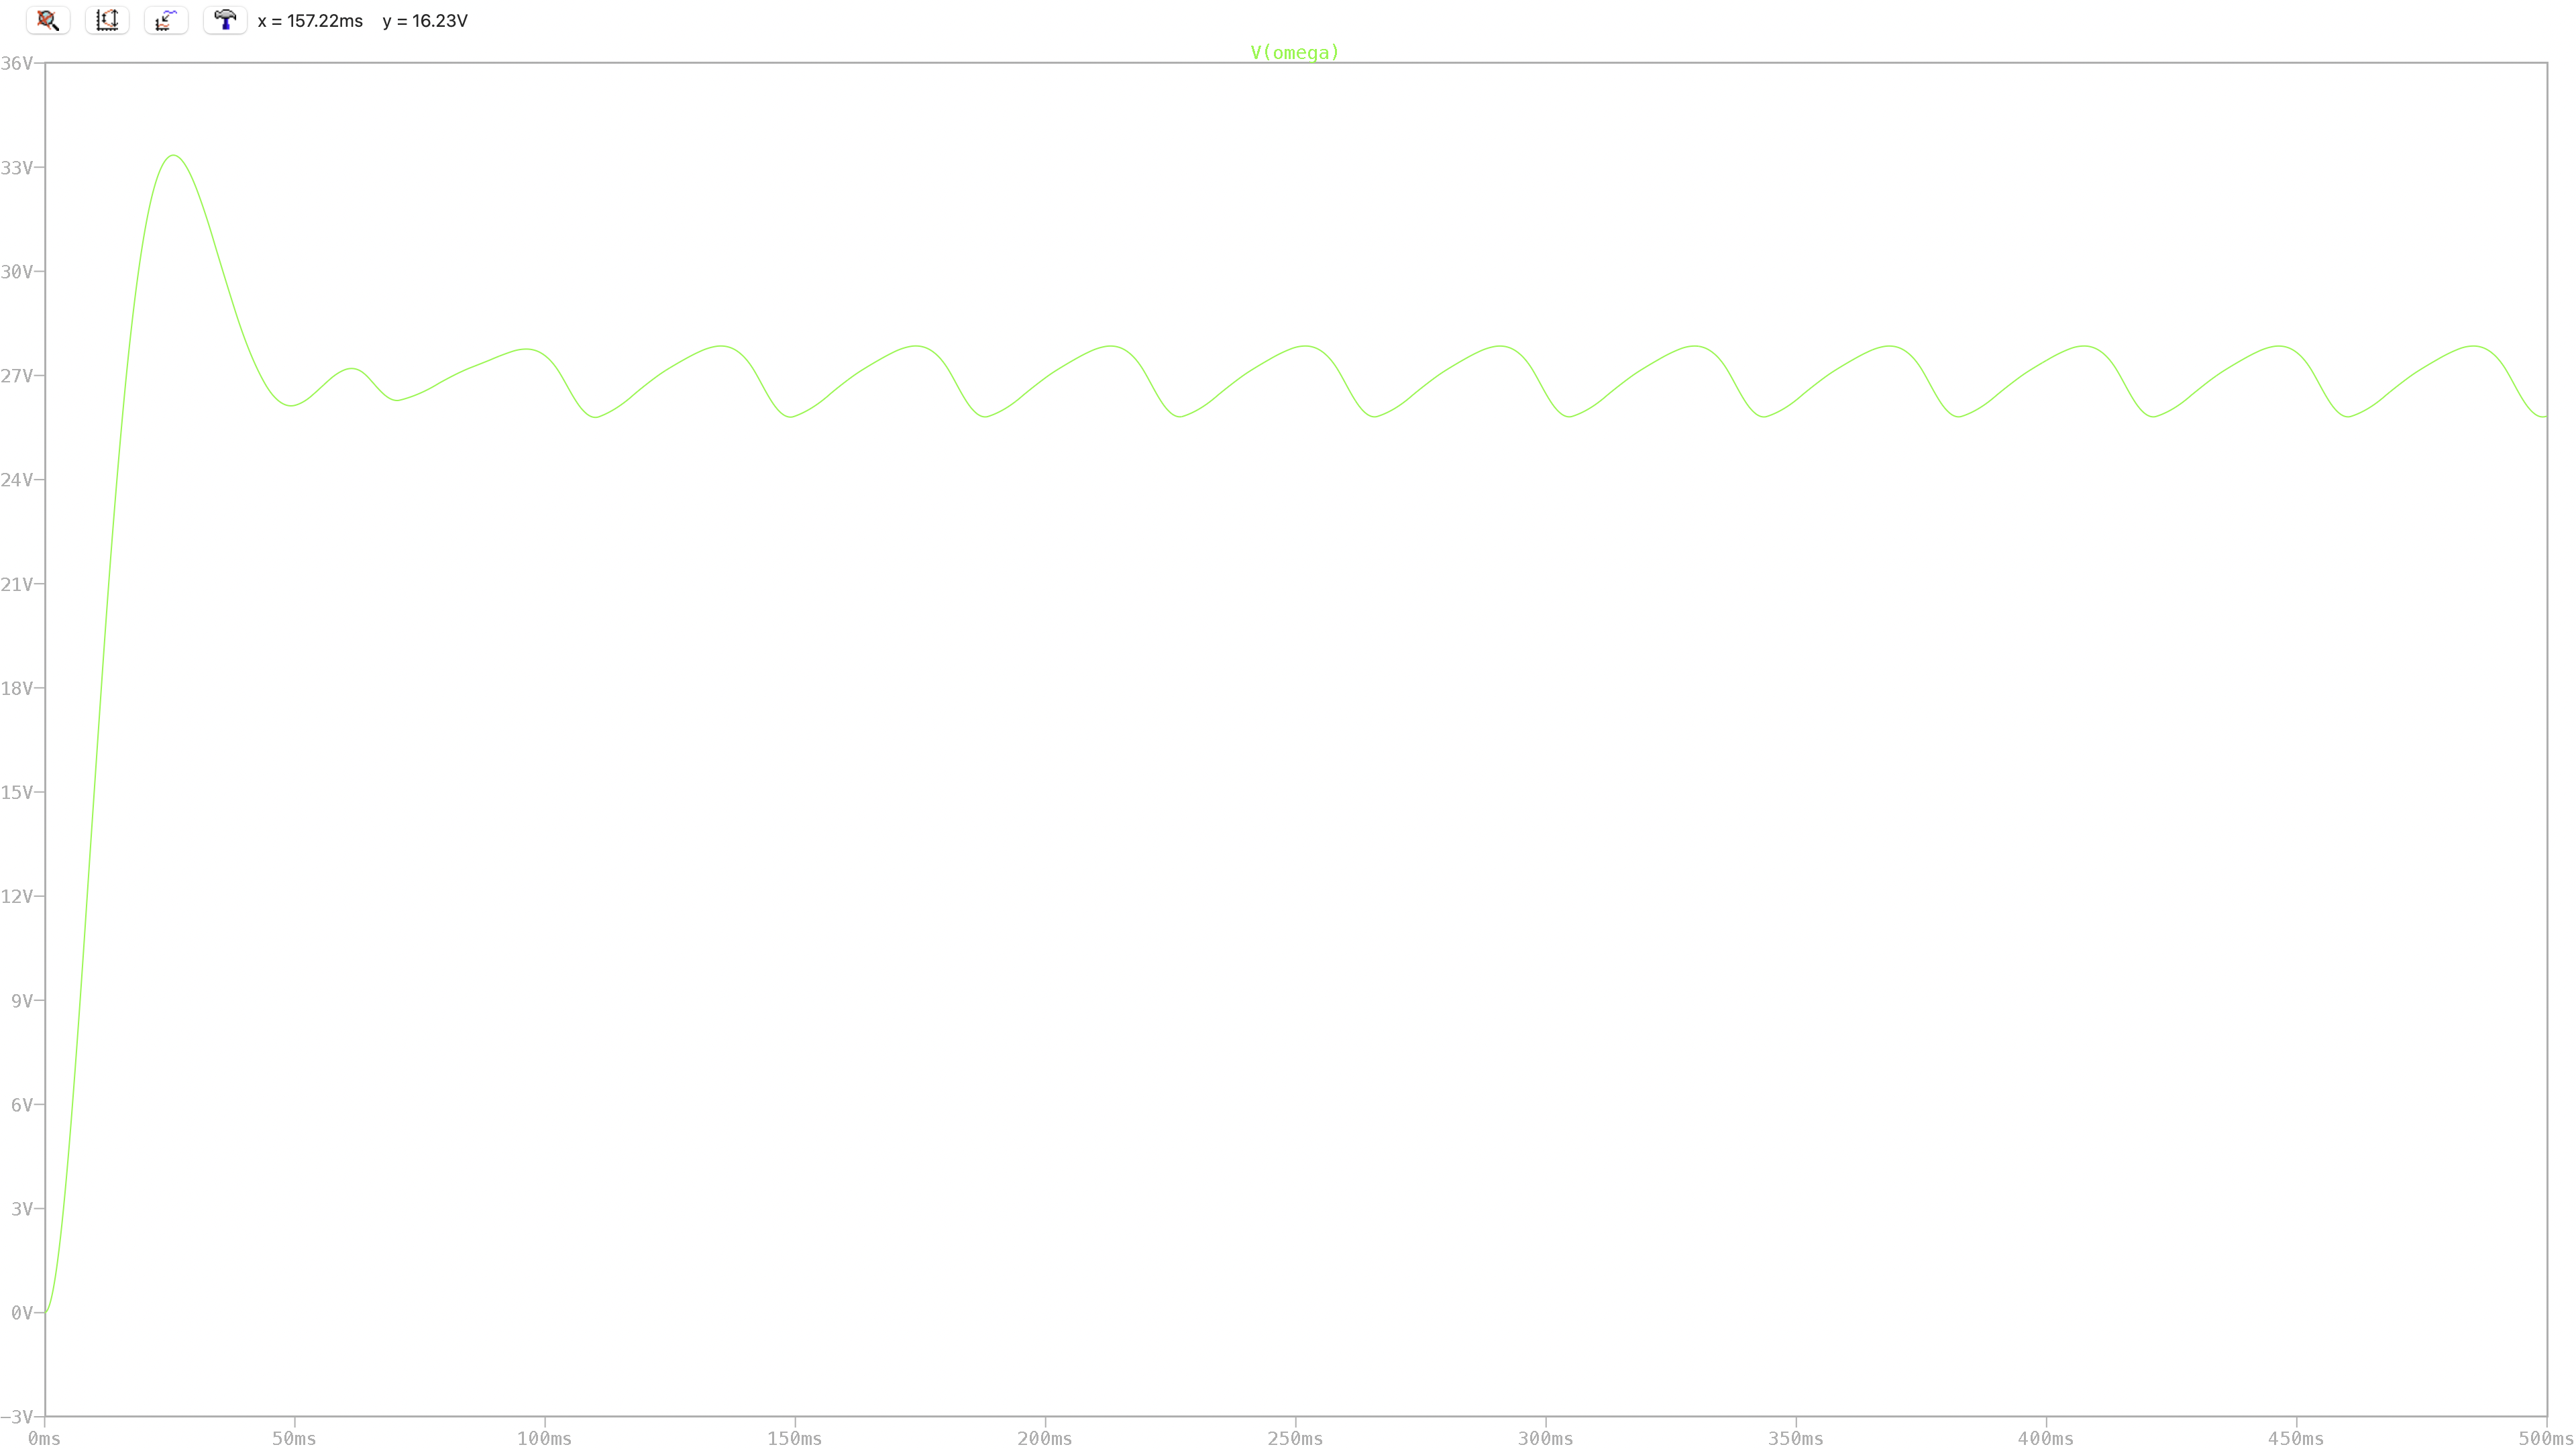
\includegraphics[width=0.8\textwidth]{images/omega_150.png}
    \caption{Przebieg prędkości kątowej silnika ($150^{\circ}$)}
    \label{fig:150_predkosc}
\end{figure}
Ograniczenie ostrych skoków momentu elektromagnetycznego stabilizuje mechanikę całego układu w stanie ustalonym. Gładsza linia przebiegu prędkości świadczy o dużo cichszej, wibrującej w mniejszym stopniu pracy napędu.

\begin{figure}[H]
    \centering
    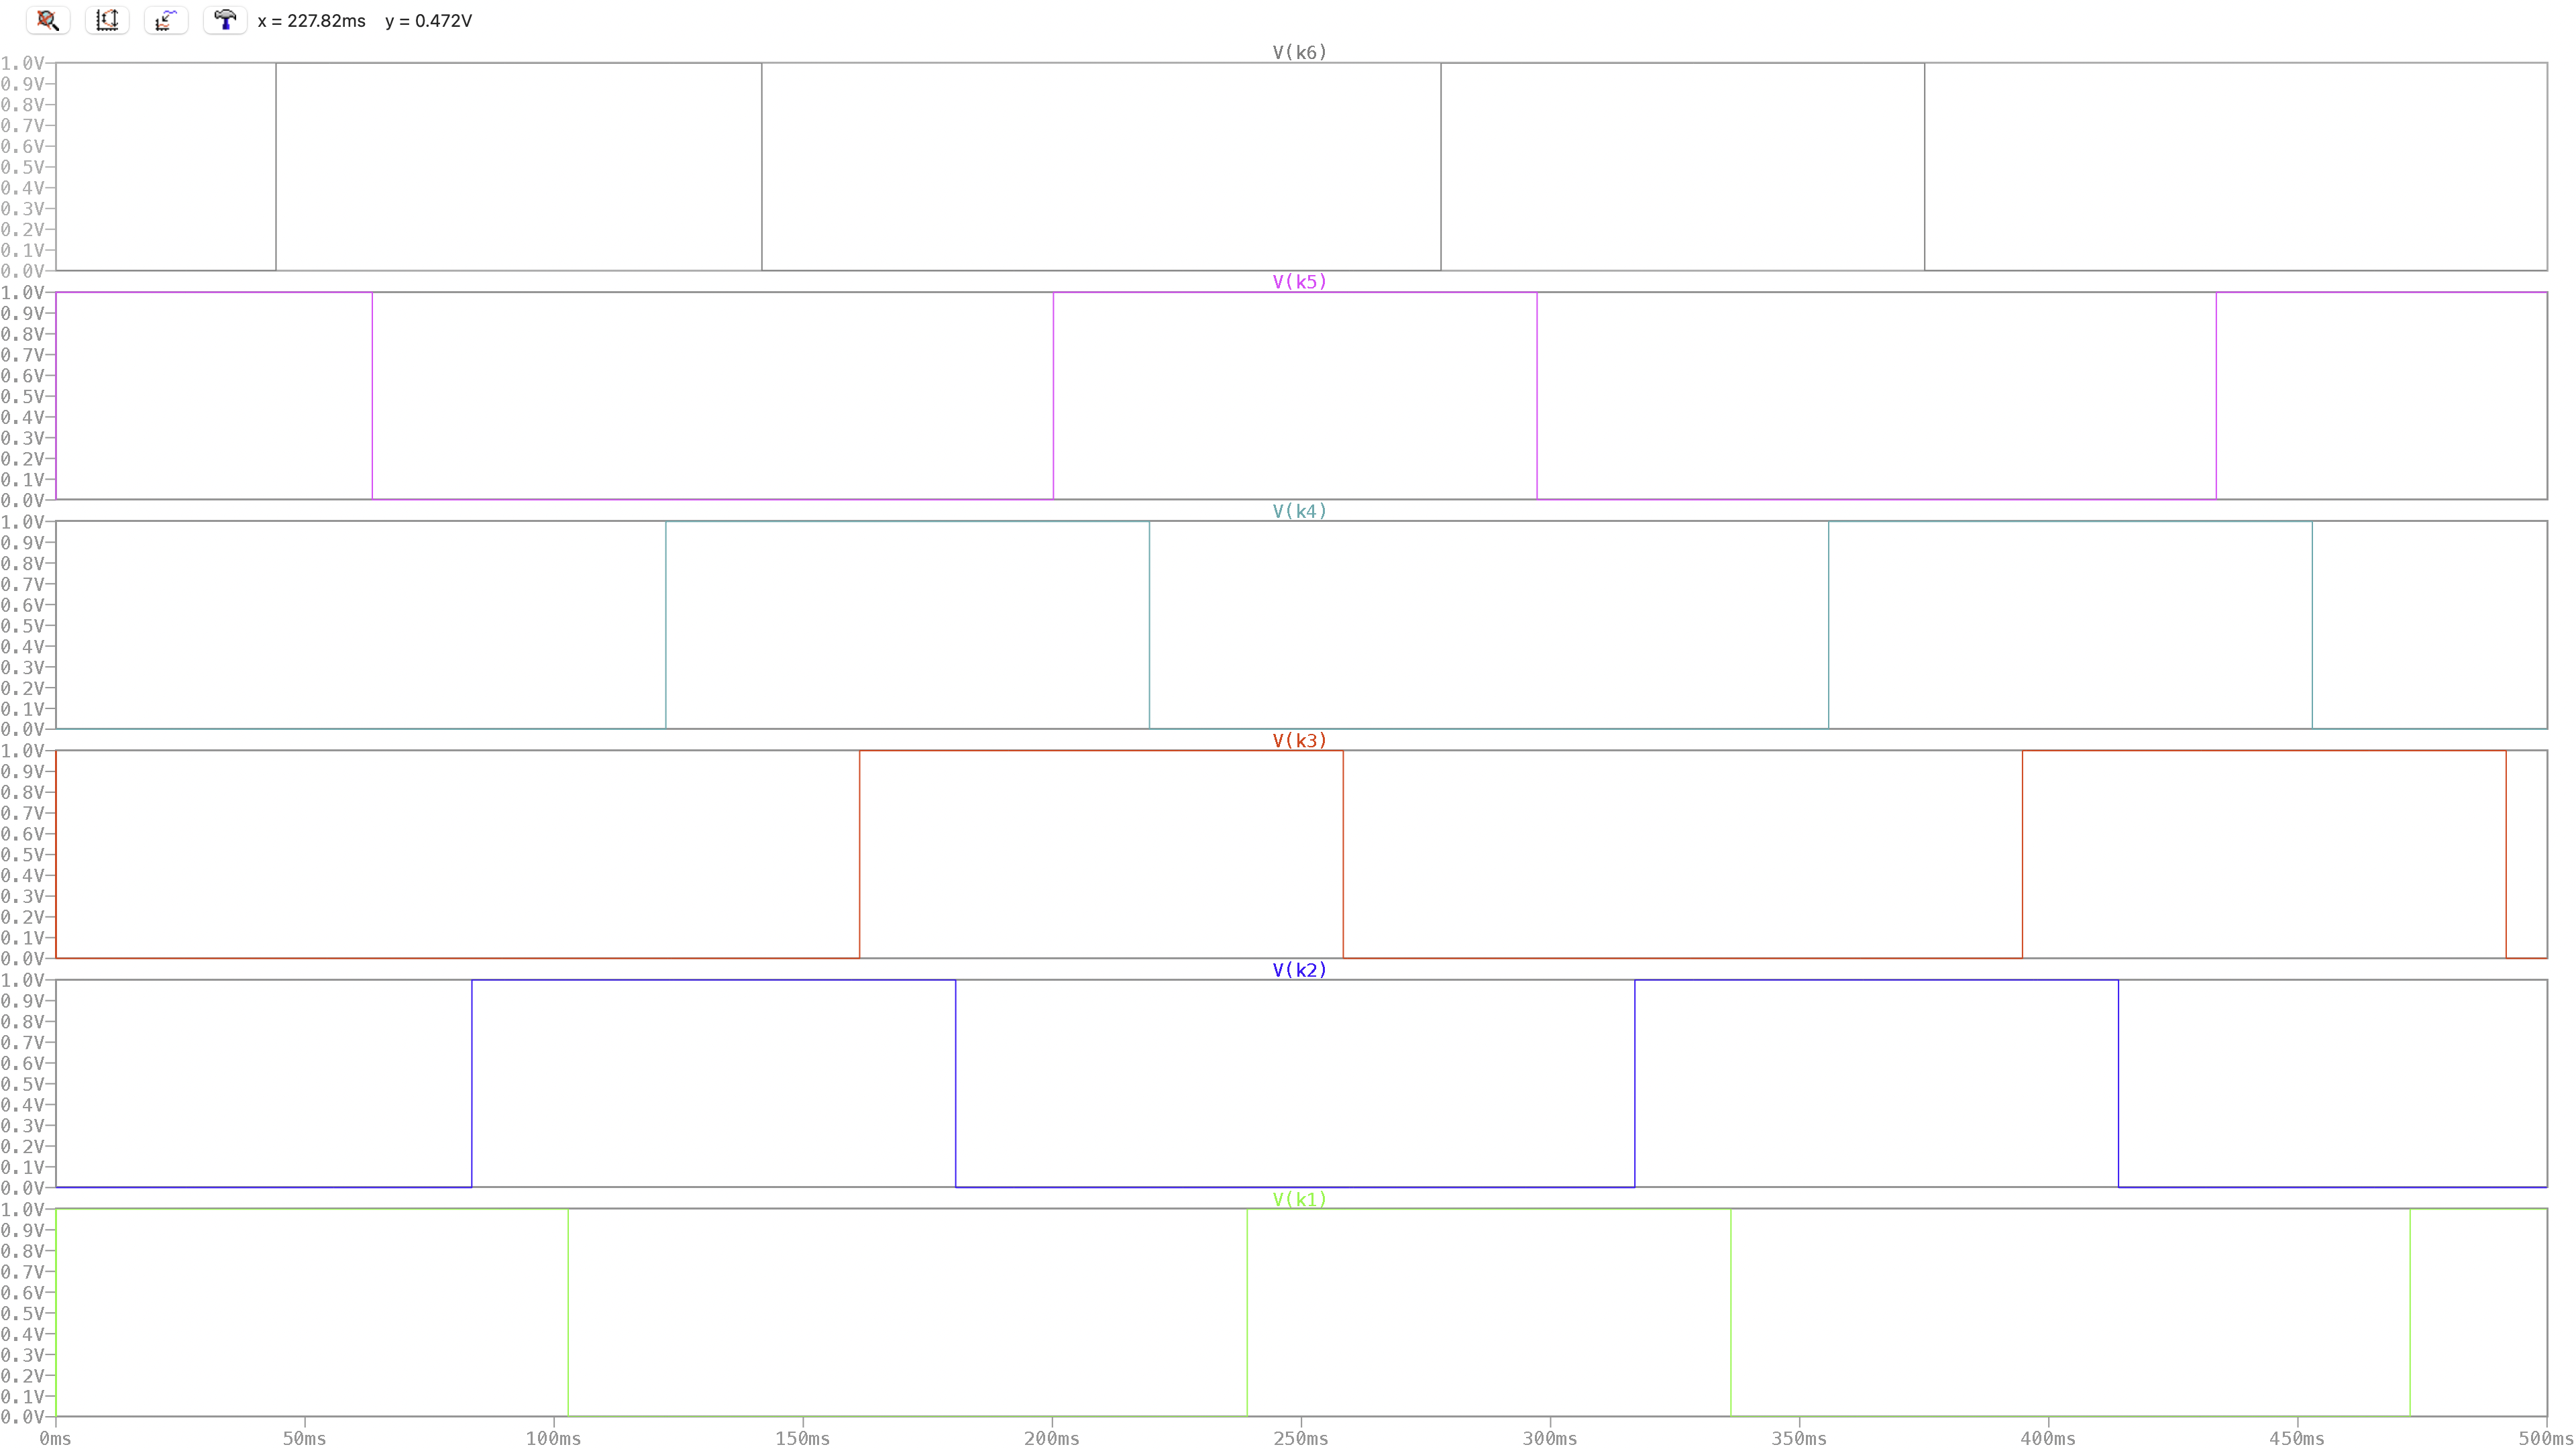
\includegraphics[width=0.8\textwidth]{images/klucze_150.png}
    \caption{Sygnały sterujące tranzystorami falownika ($150^{\circ}$)}
    \label{fig:150_klucze}
\end{figure}
Rozszerzone sygnały charakteryzują się zauważalnym zachodzeniem na siebie poszczególnych impulsów bramkowych. To zjawisko realizuje sztuczne, kontrolowane opóźnienie wyłączeń kluczy i stanowi fizyczny dowód na poprawne działanie metody miękkiej komutacji.

\subsection{Podsumowanie i porównanie metod (Wady i zalety)}
Otrzymane rezultaty symulacyjne potwierdzają stwierdzenia teoretyczne.
\textbf{Sterowanie trapezowe $120^{\circ}$ (bezczujnikowe):} Zaletą tej metody jest uproszczona konstrukcja silnika (brak czujników Halla) oraz prosta logika sterowania. Podstawową wadą, widoczną wyraźnie na sporządzonych wykresach (Rys. \ref{fig:120_moment_calkowity}), są głębokie tętnienia komutacyjne momentu obrotowego. Dodatkowo metoda ta wymusza stosowanie uproszczonych założeń przy detekcji BEMF, co objawia się szpilkami prądowymi.
\textbf{Sterowanie z rozszerzonym kątem $150^{\circ}$:} Główną zaletą jest tu znaczne wygładzenie przebiegu całkowitego momentu elektromagnetycznego (Rys. \ref{fig:150_momenty}), co podnosi kulturę pracy i zmniejsza wibracje napędu. Czas beznapięciowy dla każdej fazy skrócono z $60^{\circ}$ do $30^{\circ}$. Wadą rozwiązania jest konieczność ciągłego przeliczania wartości prędkości w celu nałożenia precyzyjnego opóźnienia na sygnały sterujące, co zwiększa złożoność algorytmiczną.

\end{document}